%\documentclass[a4paper,twoside,11pt]{report}
\documentclass{siamart171218}
%====================== PACKAGES ======================

\usepackage{ marvosym }
\usepackage{wasysym}   
\usepackage{setspace}
\usepackage{pstricks}
\usepackage{hyperref}
\usepackage{tikz}
\usepackage{xparse}
\usepackage{nicematrix}
\usepackage{stmaryrd}
\usetikzlibrary{fit}
\usepackage[english]{babel}
\usepackage[utf8x]{inputenc}
\usepackage[utf8]{inputenc}
\usepackage[english]{babel}
\usepackage{minted}
\usepackage{multicol}
\usepackage{algorithm} 
\usepackage{algpseudocode} 
\usepackage{comment}
\usepackage{hyperref}

%pour gérer les positionnement d'images
\usepackage{float}
\usepackage{amsmath}
\usepackage{hyperref}
\usepackage{hyperref}
\hypersetup{
    colorlinks=true,
    linkcolor=blue,
    filecolor=magenta,      
    urlcolor=blue,
}
\urlstyle{same}
\usepackage{graphicx}
\usepackage[colorinlistoftodos]{todonotes}
\usepackage{url}

% pour gérer les annexes 
%-------------------------------
\usepackage{appendix}
\renewcommand{\appendixpagename}{Appendices}
\renewcommand{\appendixtocname}{Appendices}
\usepackage[toc,page]{appendix}

%pour les informations sur un document compilé en PDF et les liens externes / internes
%-------------------------------
\usepackage{hyperref}
%pour la mise en page des tableaux
\usepackage{array}
\usepackage{xcolor} 
\usepackage{tabularx}
\usepackage{multirow}
\usepackage{graphicx}
\usepackage[table,xcdraw]{xcolor}

%pour utiliser \floatbarrier
%\usepackage{placeins}
%\usepackage{floatrow}
%espacement entre les lignes
\usepackage{setspace}

%modifier la mise en page de l'abstract
%\usepackage{abstract}

%police et mise en page (marges) du document
\usepackage[T1]{fontenc}
\usepackage[top=1cm, bottom=2cm, left=2.5cm, right=2.5cm]{geometry}

%Pour les galeries d'images
%\usepackage{subfig}
\usepackage{subcaption}
\usepackage{lastpage}
\usepackage{amsmath,amsfonts,amssymb}
\usepackage{fancyhdr}
\usepackage{diagbox}

%\pagestyle{fancy}
%\setlength{\headheight}{50pt}
%\setlength{\textheight}{680pt}
\usepackage{lastpage}
\usepackage{nicematrix}
%page blanche 
\usepackage{afterpage}
%abstract
\usepackage{titling}
\usepackage{lipsum}

\newcommand\blankpage{%
    \null
    \thispagestyle{empty}%
    \addtocounter{page}{-1}%
    \newpage}
    
\usepackage{afterpage}
\newcommand\myemptypage{
    \null
    \thispagestyle{empty}
    \addtocounter{page}{-1}
    \newpage
    }

\usepackage[english]{babel}
\addto{\captionsenglish}{%
  \renewcommand{\bibname}{References}
}

%--------presentation-----------
\usepackage[pdftex]{graphicx}
\newcommand{\HRule}{\rule{\linewidth}{0.2mm}}

\begin{document}
%=======Presentation========
\begin{center}
\begin{figure}[h]
    \begin{minipage}[c]{.46\linewidth}
        \centering
        \includegraphics[width=4cm]{insalogo.png} 
    \end{minipage}
    \hfill
    \begin{minipage}[c]{.46\linewidth}
        \centering
        \includegraphics[width=4cm]{ONERA_logo.png}
    \end{minipage}
\end{figure} 
\end{center}

\begin{center}
{\LARGE \textbf{Rejection method for supervised classification of plant species from passive optical remote sensing data}\\
[0.4cm] }
Léa Camusat$^1$, Eva Etheve$^1$, Julie Gonzalez$^1$ , Lila Roig$^1$ \\
$^1$ National Institute of Applied Science - Toulouse, Department of Applied Mathematics \\
\today
\end{center}
\newline \\[1cm]

%====== ABSTRACT ======
\selectlanguage{english}
\renewcommand{\abstractname}{Abstract}

\begin{abstract}
\bigskip

The identification of plant species is essential for biodiversity analysis and the monitoring of environmental degradation. Many studies have highlighted the interest of optical remote sensing to map plant species on a given satellite image. Each pixel of the satellite image can be well paired with a plant since each plant has its own spectrum. However, the performance of mapping algorithms is affected by the presence of outliers: some plant species are a minority and should not be labelled. Rejecting these outliers would reduce pixel misclassification. Five classification algorithms (Regularized Logistic Regression with l1 or l2 regularization, Linear Support Vector Machine, Radial Basis Function Support Vector Machine and Random Forest) applied on an image give a vector of probabilities that a given pixel belongs to each tree species. Unfortunately no efficient post-rejection algorithm has been developed yet in the field of hyperspectral and multispectral images. Our aim is to find relevant rejection methods which can be applied post classification on probability vectors. Boundaries between species and minor species must be rejected. We compare different clustering methods applied on probability vectors: K-means, SVM (Support Vector Machine), DBSCAN (Density-Based Spatial Clustering) and GMM (Gaussian Mixture Models).  We improve our results taking the context into account. We define qualitative and quantitative ways to evaluate the rejection performance. K-means and SVM have significant visual results as they reject some specific point of interest on the image. K-means algorithm applied on the dataset Random Forest gives the best result with a True Rejection Rate of 57\%. The False Rejection Rate obtained with K-means and SVM is quite low on every dataset, around 0.5-1\%, which means that most of the time we do not reject wrongly. Our classification assists the ONERA laboratory (National Office for Aerospace Studies and Research) in their research. For example, to quantify contaminating anthropogenic impacts in soils, the vegetation condition is analysed and it is necessary to know the species corresponding to every pixels. Further research can use our results to compare the efficiency of a rejection option performed during  classification with a rejection option performed post-classification. 

\bigskip

\textbf{keywords:} remote sensing, hyperspectral, multispectral, reject option, post classification, pdf clustering \newline
\HRule % \\[0.1cm]

\end{abstract}

%\begin{singlespace}
\section{Introduction}

As a result of the significant development of anthropic activities, we become witnesses of a worrying degradation of our environment. The impact of our activities on the planet is becoming increasingly serious. Monitoring this environmental degradation is therefore necessary in order to protect our ecosystems.

Earth observation satellites are proven to be an effective tool to study the variation of our planet. For more than forty years, the numerous sensors of  orbiting satellites have offered a wide range of spatial, spectral and temporal resolutions. The processing of this information has many applications, for example, forests can be mapped to monitor their health, determine their structure and estimate their biomass (Cf. \cite{Loureno2021BiomassEU}). Wetlands can also be mapped and classified to conserve and use the resources intelligently and evaluate the impacts of climate change and human activities on the coastline. These studies use remote sensing, which is a set of techniques used to determine remotely the properties of natural or artificial objects according to the radiation they emit or reflect. Remote sensing involves three steps: capture and recording of the radiation received, processing of the resulting data and finally analysis of these data. Here, a particular interest is given to optical remote sensing in the reflective spectral range (0.4-2.5 µm) adapted to the mapping of plant species and/or habitats. \\

To map plant species, supervised classification methods based mostly on machine learning techniques are used. However, these methods usually require a large training set of data representative of the species to be mapped, which is a problem in the field of teledetection. In the domain of teledetection, images are large and are not labelled most of the time because it can be difficult to obtain field data on all the images (for example if the areas are difficult to access). Thus, some of the species are forgotten or not enough present on the images. We can also mention the problem of mixed pixels which is inherent in remote sensing data. A pixel has a defined real size on the ground, which means that we have no finer information than this pixel and that it can be composed of several species. The efficiency of a classification algorithm depends on its ability to “trade-off the risk-coverage (RC) for higher accuracy” \cite{ran2010Noise}. A good model is supposed to assign many  features to a class and to avoid misclassification at the same time. It requires the implementation of a reject option to build a rejection class grouping pixels (representing plant species) likely to be misclassified.

A reject option in classification was first considered by \cite{5222035}, who developed a reject option based on the Bayes rule, which consists in not classifying a data point if the maximum post classification component of the probability vector is lower than a given threshold. Unfortunately, very few rejection methods have been developed in the field of hyperspectral and multispectral images. Moreover, most of the rejection methods are being applied during the classification, while we have to implement a post-classification method. For example, \cite{7326344} presents two classification methods with rejection in the field of hyperspectral images. One method consists in jointly computing context and rejection, and the other one computes them sequentially. An extra class models the probability that the classifier fails to sort a pixel into a class. These two methods applied on the dataset \textit{Avriris Indian Pines} respectively provide a non-rejected accuracy of 80\% and 76\%\ and a classification quality of 78\% and 74\%.

Our objective is to find relevant rejection methods which can be applied post classification on probability vectors. 
We consider two categories of rejection options: novelty rejection, which involves rejecting pixels that are from minority species, and ambiguity rejection, which refers to the rejection of boundaries between several species.


We use clustering techniques to implement a post-classification rejection method and classify probability vectors. One of the main advantages of clustering is that it is an unsupervised technique, that is to say we do not need the labels of the data points. Pixels are grouped by similarity, according to their probability vectors, in which each component is the probability to belong to the different species.

Clustering of probability vectors has already been investigated in several works. For example,\\ \cite{Classifier_based_affinities} aimed to classify a set of vectors. Vectors were considered as independent and identically distributed (i.i.d) samples  and their probability density function (PDF) was estimated using Gaussian Mixture Models (GMM). Then, one has to define an adequate distance measure, such as the Kullback-Leibler divergence so that clustering algorithms can be applied on probability vectors. They tested their clustering algorithm on the \textit{MoG dataset} and tunned their parameters, the best result they obtained gave a clustering error of about 15\%.

We can also mention \cite{Clustering_probability_distributions}, who estimated PDFs nonparametrically from the data and grouped them into homogeneous clusters. Several clustering algorithms were then applied, such as K-means, hierarchical and non-hierarchical methods, clustering with a bound on  cluster widths and intercluster distances.

We perform different supervised and unsupervised methods applied on probability vectors: K-means, SVM (Support Vector Machine), DBSCAN (Density-Based Spatial Clustering) and GMM (Gaussian Mixture Models).

K-means is an unsupervised partitioning-based algorithm. The main advantage of an unsupervised algorithm is that one does not need to know beforehand the labels of the data. Given a number K of clusters, K-means minimizes the distance between the data points and the cluster centers. This method cannot detect outliers; however, it can predict for new data. Rejection methods based on K-means clustering have been investigated in other works. For example \cite{6566435} used the fact that K-means computes clusters centers, thus one can predict if a point is an outlier or not by setting up a maximum distance to the cluster center. Within this distance, the point are considered close enough to be associated to the cluster. They presented the ODC algorithm (Outlier Detection and Clustering) which is based on K-means algorithm. In this algorithm a data point that is at p times the average distance away from the cluster's centroid is considered to be an outlier. To measure the efficiency of the ODC algorithm, they computed the ratio of within-class variance against the inter-class variance. Detecting and removing outliers should reduce the value of this ratio. For example, in Glass data, the value of the ratio was 0.92 and the value dropped down to 0.67 with the detection of the outliers.

DBSCAN is an unsupervised density-based algorithm. It cannot make predictions on new data, but it detects outliers. Thus, it can be directly applied to our problem \cite{dbscan}.

SVM algorithms can be considered as efficient algorithms to carry out a reject option in binary classification problems. They consist in finding a $p$-dimensional hyperplane which separates the data into classes maximizing the boundaries on both sides of the hyperplane(Vapnik rule). The rejection based on SVM models has been implemented by \cite{djeffal_2012} and \cite{Grandvalet2008}. 

GMM is an unsupervised and probabilistic soft clustering method. Since many data sets can be modeled by Gaussian Distribution, the GMM algorithm assume that the clusters come from different gaussian distributions and tries to model the dataset as a mixture of several gaussian distributions. Like K-means, this algorithm needs the number of clusters and does not require the labels of the data. However, rather than giving hard assignments into clusters as K-means, GMM gives soft assignments. This means that for each data point, GMM gives  a vector of probability that the point belongs to each class.
However, the work of \cite {deng2019selective} proposes to use a modified version of GMM to implement a post-classification rejection method to select representative paintings of an artist. Using convolutional neural network, this method first extract a content-style feature vector for each painting. Then it performs Robust Continuous Clustering (RCC) and uses an algorithm similar to GMM to reject non-representative paintings. The K-means and Agglomerative clustering methods are also used instead of RCC for comparison. The algorithm is tested on various paint databases and has a classification accuracy of about 91.42\%.

We use Python programming language and QGIS software that facilitates the visualization of species classification in space. We also carry out rejection methods with K-means, DBSCAN and SVM algorithms which are in Python's Sklearn library and implement our own GMM algorithm. Finally, we evaluate their performance and compare the  results.

%%%Agglomerative clustering is a connectivity-based method, which consists of successively grouping the closest clusters in pairs at each step, with different linkages. However, this method cannot detect outliers and cannot make prediction on new data, so it cannot be applied to our problem. 

%%%%%%%%%%%%%%%%%%%%%%%%%%%%%%%%%%%%%%%%%%%%%%%%%%%%%%%
\section{Description of the data} 
% Nommer les noms exactes des documents ? 
Within the framework of this research, all the datasets were provided by the ONERA research center. We work on an airborne hyperspectral image of a given area, which size is 2.45 km² represented by 2516 × 2473 pixels and a smaller image of size 624 × 361 pixels extracted from the original image. This smaller image allowed us to test our algorithms more quickly on a smaller dataset, the size being sometimes a problem to store the data, as is shown with \textbf{DBSCAN} algorithm. The image was preprocessed and some pixels that do not correspond to vegetation (buildings, paths, eletricity wires) or correspond to shaded pixels were discarded. These pixels were not considered as training data and we did not apply any clustering to them. We note the presence of 40\% shadow pixels on the small image and 78\% shadow pixels on the complete image.

Initially, the ONERA research center implemented five algorithms: Regularized Logistic Regression with l1 regularization (Lasso regularization) - (\textbf{RLR l1}), Regularized Logistic Regression with l2 regularization (Ridge regularization) (\textbf{RLR l2}), Linear Support Vector Machine (\textbf{SVML}), Radial Basis Function Support Vector Machine(\textbf{SVMRBF}) and Random Forest (\textbf{RF}). These algorithms were applied on the remote sensing data captured in the region of which we have the satellite image. For each pixel, the algorithms gave a vector of probabilities that the pixel belongs to each tree specie, as well as the class to which the pixel would belong according to this vector. Thus, they obtained two matrices containing the result of this first classification.
The first matrix is a 3-dimensional matrix, containing the probability vectors of each pixel. The first two dimensions of the matrix in the plane corresponding to the dimensions of the image (width \textit{w} and length  \textit{l}). The third dimension corresponds to the probability vector of each pixel and its length is equal to the number of tree species \textit{n}. The ten following species are being considered:  \\[0.1cm] 
% The third dimension corresponds to the number of classes  \textit{n} (i.e the number of plant species present on the image). Here we have the 10 following classes : \\[0.1cm]

\begin{center}
\begin{minipage}{0.4\textwidth}
\begin{flushleft} 
\begin{spacing}{0.5}
\begin{itemize}
    \item[\color{black}{--}] \textit{Platanus}
    \item[\color{black}{--}] \textit{Salix}
    \item[\color{black}{--}] \textit{Populus}
    \item[\color{black}{--}] \textit{Quercus}
    \item[\color{black}{--}] \textit{Alnus}
\end{itemize}
\end{spacing}
\end{flushleft}
\end{minipage}
\begin{minipage}{0.4\textwidth}
\begin{flushright}
\begin{spacing}{0.5}
\begin{itemize}
    \item[\color{black}{--}] \textit{Robinia}
    \item[\color{black}{--}] Grass mixtures
    \item[\color{black}{--}] Shrubs mixtures
    \item[\color{black}{--}] \textit{Reynoiutria}
    \item[\color{black}{--}] Corn crops 
\end{itemize}
\end{spacing}
\end{flushright}
\end{minipage}
\end{center}

\begin{figure}[H]
    \begin{center}
     %ne pas changer la taille de la figure !!
        \includegraphics[width=10cm]{schema_explicatif.PNG}~\\[0.1cm] 
        \caption{3D representation of the input data}
        \label{fig1}
    \end{center}
\end{figure}

A representation of the 3D matrix is provided in Figure~\ref{fig1}. Each square in the grid corresponds to a pixel of the image and the probability vector of size \textit{n} associated to a same pixel is symbolized by the set of squares colored in red. We denote $p_i$ the probability that a given pixel belongs to the class i. \\
The second matrix is a 2-dimensional matrix of width \textit{w} and length \textit{l}. For each pixel, it contains the class predicted by the algorithm according to the obtained vector of probabilities.

\bigskip

\section{Methods}
%%%%%%%%%%%%%%%%%%%%%%%%%%%%%%%%%%%%%%%%%%%%%%%%%%%%%%%

In this section, we implement several clustering and rejection algorithms on our dataset: K-means, SVM, DBSCAN and GMM.


%We use several distance metrics : 
%\begin{itemize}
    %\item[\color{black}{--}] Wasserstein
    %\item[\color{black}{--}] Kulback Leibler divergence, which represents the dissimilarity of two probability distributions. Given two probability distributions P and Q: $$D_{KL}(P|Q)=\sum_i log\frac{P(i)}{Q(i)}$$
%\end{itemize}

\subsection{Training set and context}
\subsubsection{Classification rule for the algorithms K-means and SVM}\\
\label{section:rule_selection}

\textbf{K-means} and \textbf{SVM} algorithms are two of the most used clustering algorithms. They can perform an accurate clustering; however, they cannot detect outliers. Thus, we have to build a training set and a set to be predicted so that we can perform outlier detection based on the clustering of these two algorithms.

We distinguish three categories of pixels: 
\begin{itemize}
\item{The pixels that have been well classified by the algorithms \textbf{RLR l1}, \textbf{RLR l2}, \textbf{SVML}, \textbf{SVMRBF} and \textbf{RF}, and that form a training set for the clustering algorithms \textbf{K-means} and \textbf{SVM}}
\item{The pixels that the algorithms have been unable to classify and that we have to predict on the trained models, to allocate them to a cluster or to reject them if they are outliers}. 
\item{The remaining pixels are shaded and non-vegetated pixels, they are not taken into account in the training set.}
\end{itemize} 

To determine which pixels have been well classified by the algorithms \textbf{RLR l1}, \textbf{RLR l2}, \textbf{SVML}, \textbf{SVMRBF} and \textbf{RF}, we implement three classification rules based on different hypotheses. \\

\textbf{First Hypothesis: the 0.5 rule}\\
The first assumption we can make is that a pixel has been classified correctly almost surely when the highest component of its probability vector is greater than \textbf{0.5}. There are \textbf{10 classes}, which is quite large, so this assumption seems reasonable. \\

\textbf{Second Hypothesis: the 0.5 and difference rule}\\
This rule is based on the first one: we retain pixels whose highest predicted probability is greater than 0.5. However, we include a second restriction: \textbf{the difference between the two highest probabilities} in the vector of a pixel should be higher than a certain threshold. For example, if the probability that a pixel belongs to the \textit{Platanus} class is 0.51 and that its probability to belong to the \textit{Salix} class is 0.49 we cannot be sure that there is no confusion between the two classes. Thus, the pixel will not be part of the training set and will have to be predicted by the clustering algorithms. This rule may also be relevant to reject the mixed pixels.\\

\textbf{Third Hypothesis: the cross rule}\\
Initially, the classification of trees was made with five algorithms giving the 3D matrix of probability vectors. We only retain the pixels which have been classified correctly by all algorithms and in the same class to build the training set. It corresponds to the third hypothesis. We can thus cross results between each algorithm and expect a more accurate classification.\\



\subsubsection{Classification with context}

The context should be considered when classifying and rejecting pixels. For example, pixels that are surrounded by rejected pixels are likely to be rejected as well. Furthermore, pixels that have been rejected but that are surrounded by pixels of the same class are more likely to be classified in that class. Taking context into account allows smoother classification and avoids misclassification for punctual pixels. Context can be processed post classification to improve the rejection accuracy. Two parameters must be chosen: the size of the sub-image which surrounds each pixel which was not classified, and a threshold which quantifies the proportion of pixels from the majority class of the sub-image. If this threshold is lower than the proportion of the majority class, we classify the pixel as belonging to the majority class. A pseudo code for this method is presented in the appendix \ref{Annexe:classif_context}.


\subsection{ Rejection algorithms}

\subsubsection{K-means algorithm}
\label{section:KmeansAlgo}

K-means algorithm is an unsupervised partitioning-based algorithm. \\ Given a number $K$ of clusters, K-means minimizes the distance between the data points and the cluster centers. The problem can be formulated as follows: 

\begin{equation}
\min_{A,c} \sum_{i=1}^M\sum_{k=1}^K a_{i,k} \text{ s.t. } 
\begin{cases}
      \sum_{k=1}^K a_{i,k} = 1 \forall i \in {1,...,M} \\
      a_{i,k} \in \{0,1\}
    \end{cases} 
    \label{Kmeans_pb}
\end{equation}
%  \textit{"Unsupervised clustering with E.M."})p.75,
This problem is solved by the \textbf{Expectation Maximization (EM) algorithm} (Cf. \cite{polyADD}, as described in the pseudo code in the appendix \ref{Annexe:EM_algo}).

We use the already implemented python function \textbf{K-Means} of the library \textbf{sklearn.cluster}. The metric used by this algorithm is the euclidian distance, which might be criticised given that our dataset is composed of probability vectors. Nevertheless, the advantage of K-Means algorithm is that it is a fast algorithm which can predict the cluster of new data.

We have ten different species so we want to build ten clusters with K-means. First, we train the K-Means algorithm on the training data selected by one of the above classification rules. As the K-Means algorithm does not detect outliers and predict the pixels that have been unclassified, we then implement a post clustering rejection method using the \textbf{radius} of each cluster. 

We compute the radius of each cluster, corresponding to the maximum distance between the cluster's centroid and the training data points belonging to this cluster.
The idea is the following: if a unclassified pixel $p$ falls within a distance of the radius times a given threshold ($T \le 1$) from a cluster center, we can consider that the pixel belongs to this cluster. Otherwise, if the pixel $p$ is at the border between two clusters or if it does not fall in any cluster, we reject it. The threshold $T$ has to be calibrated to find the value that will best fit our data.  If $T=1$, we consider the entire radius thus we reject less. As soon as $T$ decreases, the radius' length decreases, thus the specificity of the result increases and we reject more often as we consider that points that are at the edge of the cluster are not representative of the cluster. The pseudocode for this method is given in appendix \ref{Annexe:Kmeans_Reject}.  

To calculate the radius of a cluster or to compare the distance between a data point and the center of a cluster, we need to define a measure. Because the distance we want to measure is between two probability vectors (which sum to 1), the Euclidean measure does not appear appropriate. We decide to use the Wasserstein metric which can be taken as a reasonable distance on spaces of random variables or probability distributions \cite{givens1984class}. \\
Let $(M,d)$ be a metric space. For each $p$ with $1 \le p < \infty$, let $\mathcal{P}_p (M)$ denote the collection of all probability measures (i.e. laws) $\mu$ on (the Borel sets of) $M$ with finite $p^{th}$ moment, that is, there are some $x_0$ in $M$ such that: 
\begin{equation}
\int_{M} d(x,x_0)^p \mathrm{d}\mu(x) < \infty
    \label{eq_moments}
\end{equation}
where $d(x,x_0)^p$ is for example the p-norm $\lVert x - x_0 \rVert_p$. 
The $p^{th}$ Wasserstein distance between two probability measures $\mu$ and $\nu$ in $\mathcal{P}_p (M)$ is defined as 
\begin{equation}
W_p(\mu,\nu):=  \left( \underset{\gamma \in \Gamma (\mu,\nu)}{inf} \int_{M\times M} d(x,y)^p \mathrm{d}\gamma(x,y) \right )^{1/p} 
    \label{Wasserstein}
\end{equation}
where $\Gamma (\mu,\nu)$ is the set of all couplings $\mu$ and $\nu$. 

\subsubsection{SVM}
We assume that the data can be linearly separated. Pixels which are rejected are those which are in the gap between the two boundaries. 
This problem can be extended to a multi-classification task. There are several methods such as OVR (One vs the Rest) and OVO (One vs One). OVO consists in calculating hyperplanes two by two. In our classification problem, we have optimized 45 hyperplanes (K(K-1)) with K, the number of classes. Due to the asymmetry of the dataset used to optimise each hyperplane, OVR is considered to increase the bias, as each hyperplane is built to separate one class and the nine other classes \cite{djeffal_2012}. \\

We implement a calibration method, which is based on the \textit{decision\_function} of the method \textit{svm} in Sklearn. The decision function is computed according to the votes and can be seen as a way to measure the confidence on the prediction. We obtain a matrix containing each probability of the respective label for each pixel ($pixel\_to\_predict \times 10~\text{classes matrix}$), which can be considered as a way to measure the confidence in the prediction. 

We implement the rejection method shown in Algorithm \ref{Annexe:SVM_reject}.

The specificity of this algorithm is that we decide to set a rejection rate instead of determining a threshold. We predict only pixels which are not in the training set based on the rules of preclassification. All pixels that have a relative difference of decision function lower than the median (or the 3rd quartile) of these relative differences must be rejected, as this indicates that the classifier did not decide between two classes, and that we are in an undecision area (Figure \ref{fig2}). 



\begin{figure} [!h]
\begin{center}
\includegraphics[width=0.7\textwidth]{undecision boundary svm.PNG}~\\[1cm]
\caption{Undecision area in OVO}
\label{fig2}
\end{center}
\end{figure}


\subsubsection{DBSCAN algorithm}

DBSCAN, or Density-Based Spatial Clustering of Applications with Noise, is an unsupervised machine learning algorithm. The main asset of using an unsupervised algorithm on our dataset is that we do not need to know in advance the labels. DBSCAN is well suited for problems which requires minimal domain knowledge to determine the input parameters. For example, unlike K-means, DBSCAN does not need the number of clusters beforehand.
We use an already implemented function from library \textbf{sklearn.cluster} called \textbf{DBSCAN}. As for many machine learning algorithms, the behavior of the model is dictated by several parameters. For this algorithm, the three most important parameters are $eps$, $min\_samples$, $metric$. The choice of these parameters is explained below. \newline

\textbf{Definition and Choice of $eps$}: Two points are considered as neighbors if the distance between them does not exceed the threshold epsilon. This parameter is the most important one since it provides the condition for two points to be considered in the same cluster. We can find a suitable value for the \texttt{eps} parameter by calculating the distance between $P$ and its closest neighbour $P'$, for each point $P$. After sorting these values, we obtain a plot that shows the change of the distance between two close points. Then, we look where the slope soars and select the corresponding epsilon. In a more quantitative way, this variation corresponds to the point where the curve has a change in slope of at least 1\%. To compute these values, we used the function $NearestNeighbors$ from the library sklearn.neighbors. An illustration of this procedure is given in Figure \ref{fig3}. \newline

\begin{figure}[h!]
\begin{center}
\includegraphics[width=0.7\textwidth]{epsilon.png}~\\[1cm]
\caption{Points sorted by distance to the second nearest neighbor, best epsilon value found for 0.04}
\label{fig3}
\end{center}
\end{figure}

%\texttt{eps} does not give the maximal distance between two points within a cluster.

\textbf{Definition and Choice of $min\_sample$}: This parameter gives the minimum number of neighbors a given point should have to be considered as a core point. The point itself is taken into account in the setting of $min\_sample$. By default, the parameter is set to $2$ but by increasing its value we can make sure that we find the number of clusters in the database. The more $min\_sample$ increases the more we constrain the algorithm since a point $P$ is considered to be core point if it has at least $min\_sample$ number of points in its neighborhood. This parameter varies depending on the sample. \newline

\textbf{Choice of $metric$}: As DBSCAN computes distances between points in the database, it is important to decide how to evaluate these distances. The results can vary significantly depending on the metric used. We choose different metrics allowed by the function $DBSCAN$ and compare the number of rejected pixels they give. \newline

Once these parameters are chosen, the DBSCAN algorithm provides the clusters it has found while detecting the anomalies, in our case the pixels that are in the margin. The advantage here is that DBSCAN directly gives the pixels to be rejected by giving the label \textit{-1}. To avoid a kernel crash because of the size of the dataset, it can be better to apply this function to smaller parts of the image. A pseudo-code of the algorithm is provided in appendix \ref{algo:DBSCAN}.

\subsubsection{Reject option algorithm using GMM}
\label{section:Reject_maultivariate_gaussian}

In this section, we focus on a rejection method using multivariate Gaussian distribution and comparable to a modified GMM algorithm. The reject option occurs after a classic clustering algorithm such as K-means or GMM. To do so, we rely on the paper \cite {deng2019selective} which implements a rejection method in the case of the classification of paintings. \\

Adopting the notations of the paper, we denote  $U = \left\{ u_i |1 \le i \le n 
\right\}$ the set of probability vectors where $u_i \in \mathbb{R}^{D}$ is the vector containing the probabilities that pixel $i$ belongs to each class ($D = 10$ classes) and $n$ is the total number of pixels. We assume that the elements in cluster $U_M$ are mutually independent and obey the Gaussian distribution. \\
A clustering algorithm is then applied to all data that are not shadow pixels. In opposition to the rejection method presented in section \ref{section:KmeansAlgo}, the clustering algorithm is also applied to the unclassified pixels according to the classification rules presented in section \ref{section:rule_selection}. \\
As the clusters are assumed to be Gaussian, the data is renormalized. Moreover, it seems appropriate to apply the GMM clustering algorithm (using the already implemented Python function) which also assumes that the clusters are Gaussian. In a second phase, we apply the K-means clustering algorithm for comparison. \\

For each cluster $M$, we formulate the class-conditional-probability density of probability vector $u_i$ as 


\begin{equation}
    \mathbb{P}(u_i|M) = \frac{1}{\sqrt{(2\pi)^D det(\Sigma_M)}} e^{-\frac{1}{2}(u_i -\mu_M)^T \Sigma_M^{-1}(u_i - \mu_M)} 
    \label{class_condi_pb1}
\end{equation}

where $\mu_M$ and $\Sigma_M$ are the mean and the covariance matrix of cluster $M$. Thus, we can obtain the probability $\mathbb{P}(M|u_i)$ defined by:

\begin{equation}
    \mathbb{P}(M|u_i) = \frac{\mathbb{P}(u_i|M)\mathbb{P}(M)}{\mathbb{P}(u_i)}
    \label{class_condi_pb2}
\end{equation}

which indicates the probability of $u_i$ belonging to cluster $M$, \\
where 

\hspace{-0.9cm}\begin{minipage}{.40\linewidth}
\begin{equation}
    \mathbb{P}(u_i) =  \sum_{m \in clusters} \mathbb{P}(u_i|m)\mathbb{P}(m)
    \label{precision1}
\end{equation}
\end{minipage} 
\begin{minipage}{.56\linewidth}
\begin{equation}
    \text{and~~~}
    \mathbb{P}(M) = \frac{\textit{number of pixels in cluster M}}{\textit{total number of pixels}}
    \label{precision2}
\end{equation}
\end{minipage} \hfill
\bigskip

Therefore, a pixel which is represented as $u_i$ classified to cluster $M$ will be rejected if $ \mathbb{P}(M|u_i)$ is not higher than a threshold $T$, which means pixel $u_i$ is more likely to be an outlier of cluster $M$.

Once this rejection is completed, we cluster the data again, modifying the probability
distribution of each cluster. The cluster-rejection process is repeated until the stop criterion is met. The pseudocode for this method is shown in the appendix \ref{Annexe:GMM_reject}. We use the python function \textbf{multivariate\_normal.pdf} from \textbf{scipy.stats} to compute  $\mathbb{P}(u_i|M)$. 

\subsection{Methods to evaluate the rejection performance}
\subsubsection{Visual assessment of performance}
Some areas in the image must be rejected by our algorithms. They correspond to specific areas such as the island, the fallow land, remaining non-vegetated or shaded pixels as well as mixed pixels, electricity lines, or paths. These areas are supposed to be rejected as their spectrum is different than the species we want to classify, as we can see on Figure \ref{spectrum}. 

\begin{figure}[H]
    \centering
    \includegraphics[width=16cm]{images/refl.png}
    \caption{Spectrum of the species}
    \label{spectrum}
\end{figure}

We visually assess the performance of our algorithm in QGIS. On Figure \ref{to_be_rejected} the elements we should reject are circled in red. 

\begin{figure} [H]
    \centering
    \begin{tabular}{cccc}
        \includegraphics[width=0.3\textwidth]{images/electric_line_field.png} &
        \includegraphics[width=0.3\textwidth]{images/island.png} &
        \includegraphics[width=0.3\textwidth]{images/dirt_road.png} \\
        \textbf{(a)}  & \textbf{(b)} & \textbf{(c)}  \\[6pt]
    \end{tabular}
    \begin{tabular}{cccc}
        \includegraphics[width=0.3\textwidth]{images/borders.png} &
        \includegraphics[width=0.3\textwidth]{images/field.png} \\
        \textbf{(d)}  & \textbf{(e)}  \\[6pt]
    \end{tabular}
    \caption{ \textbf{(a)} Electricity line
    \textbf{(b)} Island
    \textbf{(c)} Dirt road crossing a field
    \textbf{(d)} Borders between two species
    \textbf{(e)} Fallow land}
    \label{to_be_rejected}
\end{figure}



\subsubsection{Field data and performance}

Biodiversity data are collected in the field in 391 areas by specialists. These areas are listed in polygon masks and can be visualized in QGIS in the Figure \ref{masks} and extracted using rasterio in the Figure \ref{polygon}. Each polygon is associated to a plant species. We use these labelled data to evaluate the performance of our rejection methods. Specialists identify 17 plant species. In our algorithms, only ten types of plants must be classified, so the seven remaining classes should be rejected. 

\begin{minipage}{0.44\textwidth}
\begin{figure}[H]
    \centering
    \includegraphics[width=6cm]{mask.PNG}
    \caption{Visualisation of masks on QGIS}
    \label{masks}
\end{figure}
\end{minipage}
\begin{minipage}{0.44\textwidth}
\begin{figure}[H]
    \centering
    \includegraphics[width=6cm]{polygone.png}
    \caption{Extraction of a polygon using rasterio on Python}
    \label{polygon}
\end{figure}
\end{minipage}

\subsubsection{Predict rejection of a known class}
To evaluate the rejection performance of our algorithms we build a new dataset, in which we delete one tree species and we perform the rejection method on this new dataset. If the rejection method is efficient we should observe that the pixels that were previously classified in the considered tree species should be rejected. We use two datasets to carry out these tests: 
\begin{itemize}
\item{two datasets built with the algorithms RLR and SVM in which the \textit{Platanus} tree species has been deleted}
\item{two datasets built with the algorithms RLR and SVM in which the \textit{Reynoiutria} tree species has been deleted}
\end{itemize} 

These tree species were chosen because their spectra are those that are the furthest from the other species.
We take the example of the dataset without the Platanus specie. 
First, we perform the rejection method on the new dataset as usual, except that we now have nine classes. Then, in the former dataset, in which \textit{Platanus} was not deleted, we find the coordinates of Platanus pixels that were part of the former training set. The reason is that, those pixels were selected by the \textbf{0.5 rule} or the \textbf{0.5 and difference rule} and were considered well classified. Next, we verify whether or not at these coordinates, the rejection method has rejected the pixels. We compute the \textbf{True Rejection Rate}:

\begin{equation}
    TRR = \frac{\#(\text{rejected pixels} \cap \text{platanus pixels})}{\#\text{platanus pixels}}
    \label{TRR_platanus}
\end{equation}

\subsubsection{Performance evaluation criteria}
%%%%%%%%%%%%%%%%%%%%%%%%%%%%%%%%%%%%%%%%%%%%%%%%%%%%%%%

 
%\begin{itemize}
%\end{itemize} 
We aim to have an overview of the different methods used to quantify the quality of a rejection method. There is no method of assessment commonly used to assess the performance of a classification method with a reject option. We also describe the main indicators and recommendations about the choices of indicators which ensure the validity of the rejection method used.
A good indicator should take into account the accuracy of the rejection and the ability of the model not to reject too much. 

According to \cite{condessa2017Performance}, a good performance measure must follow these three properties: \\
1) to be a function of rejection rate \\
2) enable a comparison of rejection methods using the same or different rejection rates.\\
3) to be maximum (and respectively minimum) for a rejection algorithm with the highest  (and respectively lowest) reliability. 

Indicators are sorted into three types \cite{condessa2017Performance}: measure of the accuracy of classification of non rejected samples, measure which deals with the quality of the rejection and measures of global efficiency in terms of accuracy and rejection. The most common indicators are also presented by \cite{guichard2010nouveau}. The following indicators are adapted to our problem to measure of quality of rejection :

TRR(true rejection rate) = $\frac{\text{true rejected}}{\text{items to be rejected}} $

FRR(false rejection rate) = $\frac{\text{false rejected}}{\text{items not to be rejected}}$

NRA(non rejected accuracy)=$\frac{\text{well-classified} \cap \text{non-rejected items}}{\text{items not to be rejected}}$

\section{Results} 

\subsection{Results of K-means clustering}
\label{Kmeans_part}

\subsubsection{Performance of K-means clustering on the training data}
First, we evaluate the performance of K-means on the training data. As we consider this data as being labelled, we can compute the purity metric (equation \ref{purity}). This external metric maps the clusters given by K-means to the real labels. First, a confusion table is built. The table has two entries, on the columns there are the real labels (i.e., the plant species) and on the rows the clusters given by K-means. For each tree species, the table counts the number of pixels that have been classified in the different K-means clusters. Then, we map each species with the cluster in which the maximum number of pixels has been allocated. For example, the confusion Table \ref{confusion_table_rlr1} was obtained using the dataset \textbf{RLR l1}. The clustering performs well since each species corresponds to a unique cluster.

We evaluate the performance of K-means to allocate each species to a unique cluster, that is to say, for each column $T^j$ of the confusion table $T$ we compute the following ratio: 

\begin{equation}
    P_j = \frac{max(T^j)}{\sum_{i=1}^{n}T^j_i} \text{, where $n$ is the number of clusters}
    \label{reussite_Kmeans}
\end{equation}
 
Finally, we compute the purity metric on the whole result: \\[-0.69cm]
\begin{equation}
    purity = \frac{1}{N}\sum_{j=1}^{n}max(T^j)
    \text{, where $N$ is the total number of pixels in the training set}
    \label{purity}
\end{equation}
The purity coefficient belongs to $[0,1]$, the closer it is to 1, the more accurate the clustering. 
\begin{table}[h!]

\centering
\caption{Confusion Table of K-means clustering on the dataset \textbf{RLR L1} } 
\begin{tabular}{|c ||c c c c c c c c c c|} 
 \hline
  & \multicolumn{10}{|c|}{Real species}\\
 \hline
  clusters & 1 & 2 & 3 & 4 & 7 & 9 & 13 & 14 & 15 & 16 \\
 \hline\hline
 0 & 17 & 0 & 0 & 0 & 0 & 0 & 336 & 181710 & 0 & 0 \\
 \hline
 1 & 0 & 0 & 0 & 0 & 0 & 0 & 0 & 0 & 0 & 244589 \\
 \hline
 2 & 17 & 35478 & 30 & 0 & 5 & 22 & 135 & 35 & 0 & 1 \\
 \hline
 3 & 24 & 0 & 185082 & 0 & 0 & 3 & 50 & 6 & 3 & 27 \\
 \hline
 4 & 82 & 0 & 36 & 103861 & 4 & 20 & 0 & 16 & 0 & 1 \\
 \hline
 5 & 89 & 0 & 99 & 0 & 143055 & 7 & 17 & 134 & 3 & 14 \\
 \hline
 6 & 2 & 0 & 0 & 0 & 0 & 68662 & 0 & 1 & 0 & 12 \\
 \hline
 7 & 6 & 0 & 0 & 0 & 0 & 0 & 218359 & 0 & 0 & 37 \\
 \hline
 8 & 105248 & 0 & 0 & 0 & 0 & 0 & 0 & 0 & 0 & 28 \\
 \hline
 9 & 43 & 0 & 0 & 0 & 0 & 0 & 1 & 7 & 26668 & 2 \\
 \hline 
\end{tabular}
\label{confusion_table_rlr1}
\end{table}


We determine the optimal rule for each dataset to build its training set. 
We vary the value of the threshold that we use to build the training set with the \textbf{rule05diff} and we compute the \textbf{purity metric}. 
We recall that if the difference between the two highest probabilities in the vector of a pixel is lower than the given threshold, then the pixel will not be part of the training set because there might be a confusion between two classes. So, the higher the threshold is, the better the purity is but also the smaller the obtained training set is. Thus, it is important to optimize this threshold. Ideally, we want K-means clustering to map each species to a unique cluster, which corresponds to a purity metric of 1. However, we also wish for the threshold to be as small as possible, so that the training set contains as many correctly classified pixels as possible. So, the rule is considered optimal when the chosen threshold gives a purity equal to 1 and is as small as possible. 

\begin{figure}[H]
    \centering
    \includegraphics[width=10cm]{images/purity_kmeans.png}
    \caption{Variation of purity metric according to the value of the threshold}
    \label{purity}
\end{figure}

We observe that for K-means clustering, the optimal rules to build our training sets are: 
\begin{itemize}
\item{\textbf{the 0.5 rule with a difference of 0.08} for the datasets \textbf{RLR1} and \textbf{RLR2}}
\item{\textbf{the 0.5 rule with a difference of 0.05} for the dataset \textbf{SVM linear} and \textbf{RF}}
\item{\textbf{the 0.5 rule with a difference of 0.07} for the dataset \textbf{SVM rbf}}
\end{itemize} 
Later, we run all our test with K-means on the datasets built with the above rules.

\subsubsection{Performance of K-means clustering on the test data}
Now that we have built the optimal training dataset, we evaluate the rejection accuracy of K-means. We analyse visually the map for points of interests, and use the two methods previously introduced with the labelled polygons and the missing class.\\

\textbf{Visual assessment on the map}\\
For each dataset, we plot the map obtained after clustering and rejection (figure \ref{map_RLR1}) and we take a closer look at some specific areas. 


\begin{figure}[H]
    \centering
    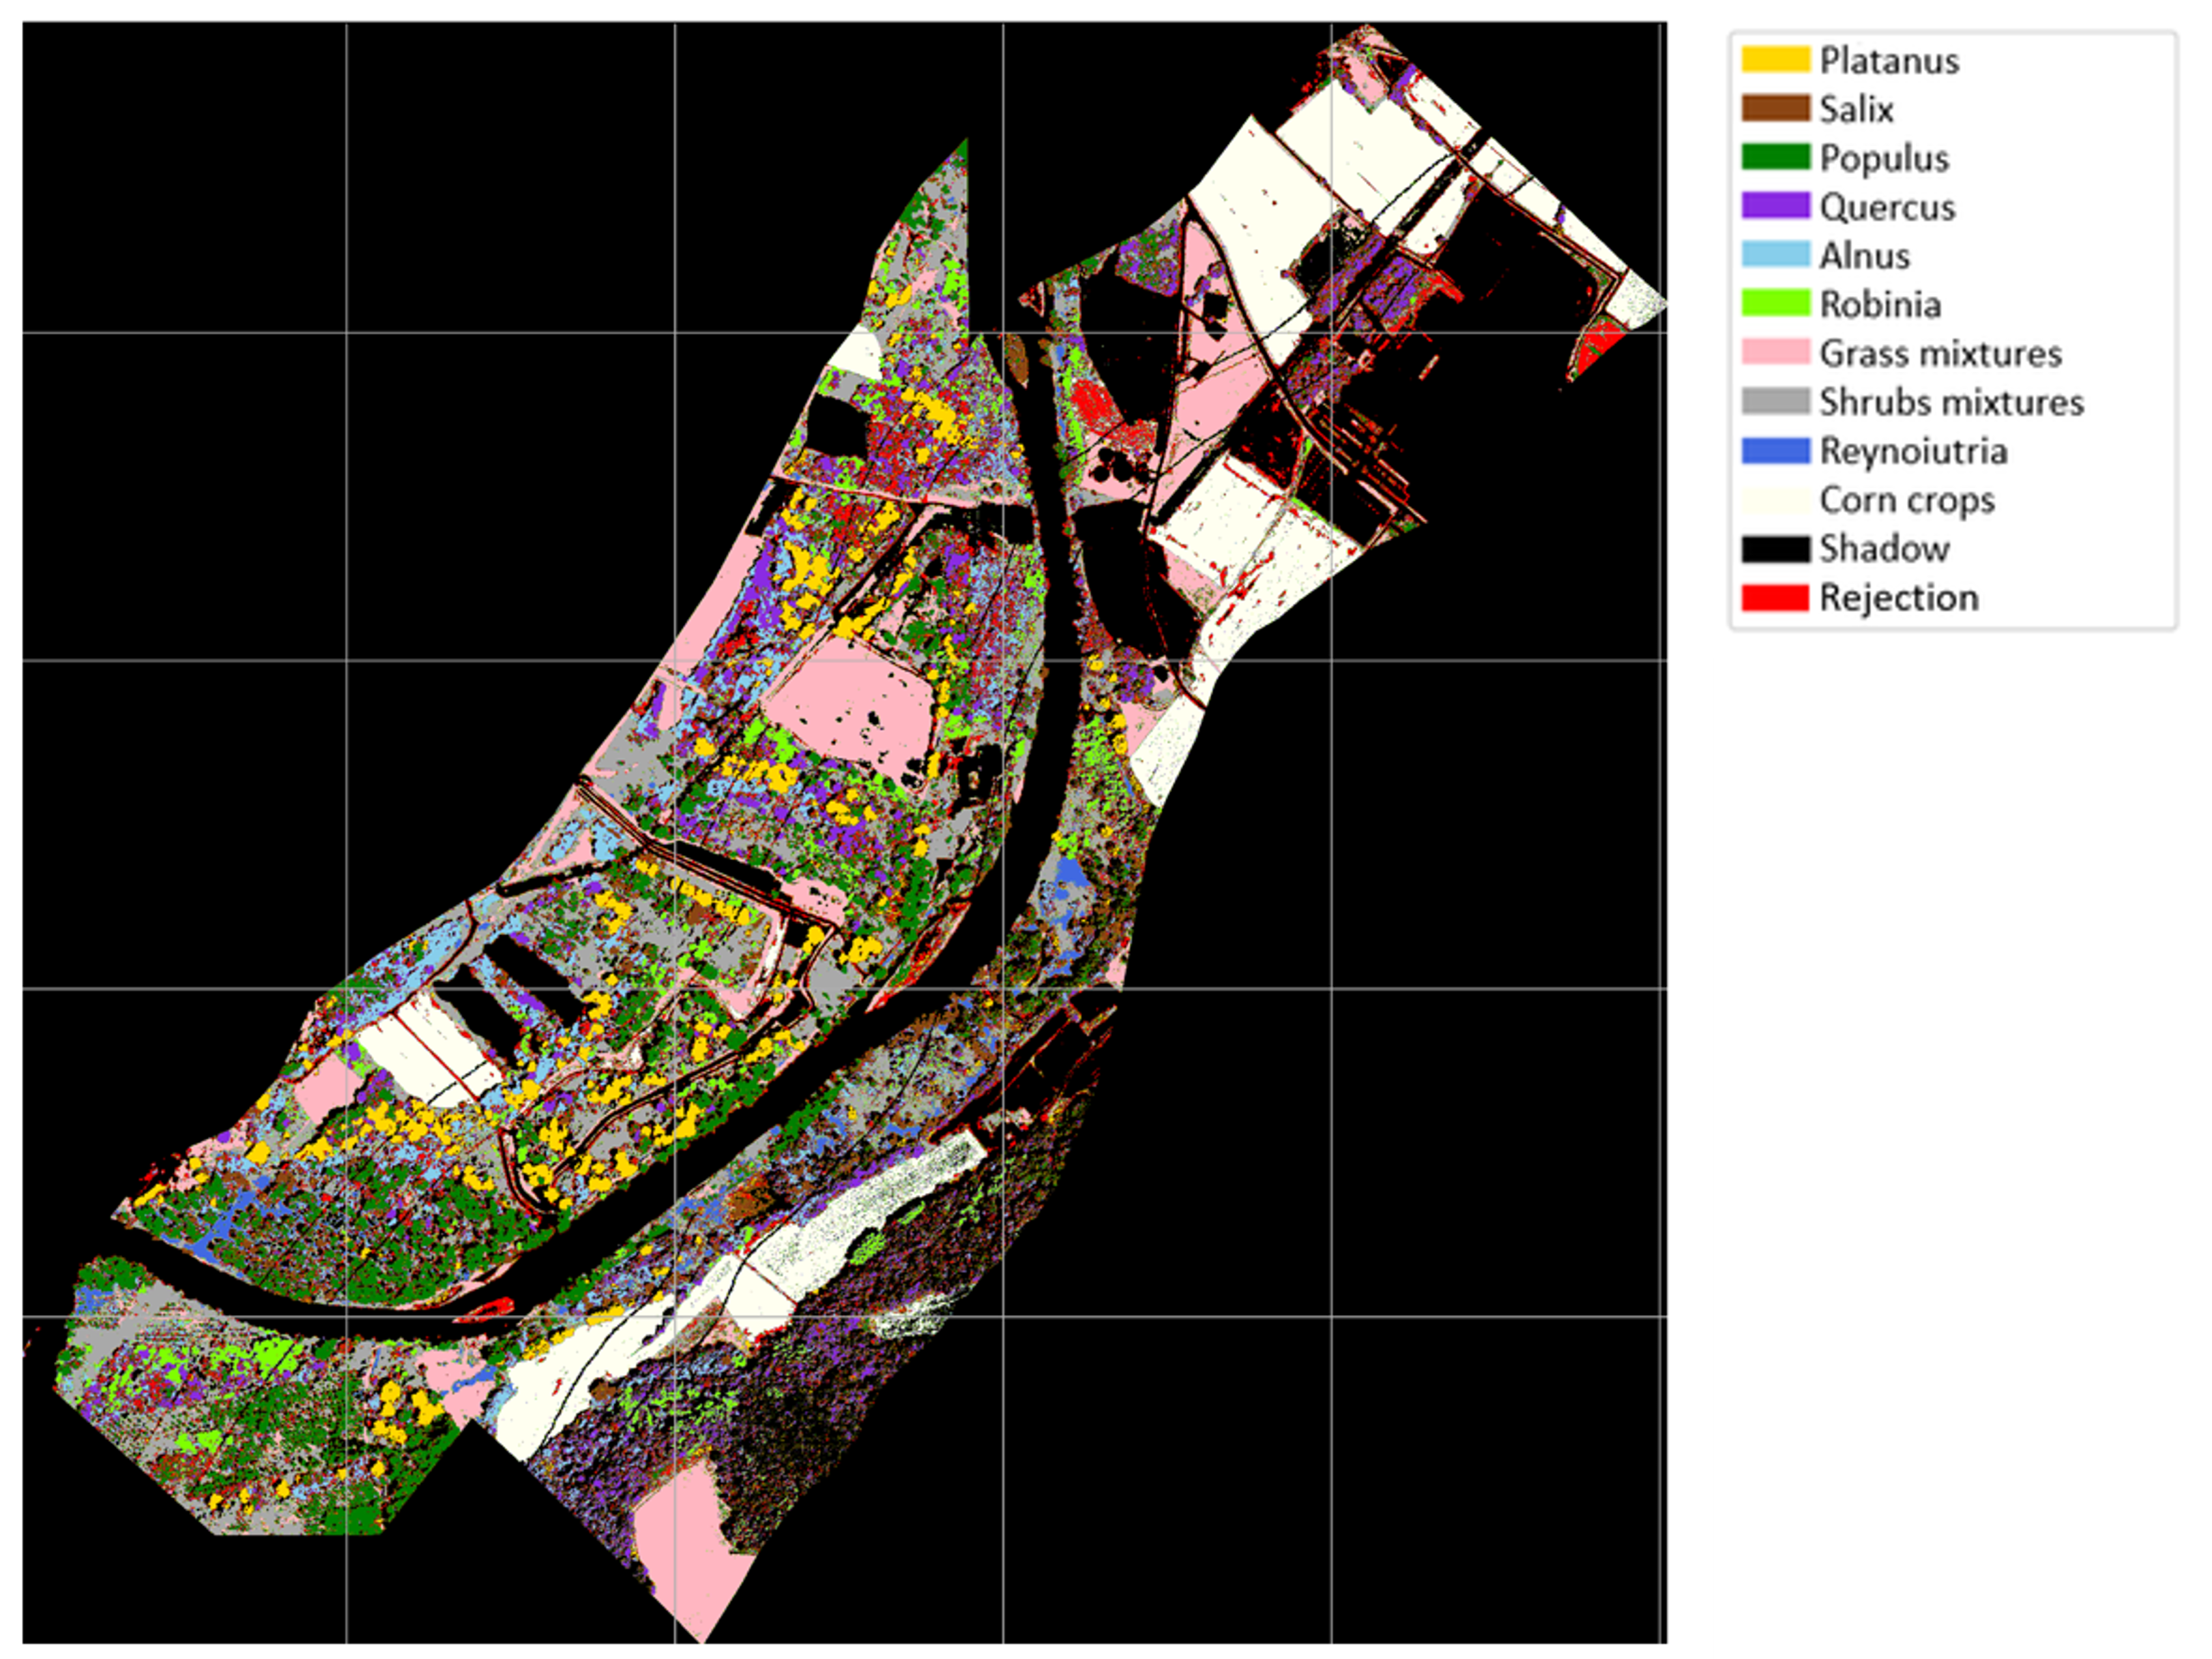
\includegraphics[width=16cm]{images/lrl1T08_rule05diff_clustering_mirror.png}
    \caption{Map after clustering and rejection with K-means on the dataset RLR l1}
    \label{map_RLR1}
\end{figure}

Table \ref{visual_assessment_kmeans} summarizes the areas of interest rejected by K-means in the different datasets. 

\begin{table}[h!]
\centering
\begin{tabular}{|c ||c c c c c|} 
 \hline
    & RLR l1 & RLR l2 & SVM linear & SVM RBF & RF \\
 \hline\hline
Electricity line & $\times$ & \checkmark & $\times$ & $\times$ & $\times$ \\
 \hline
 Fallow land & \checkmark & partly & \checkmark & \checkmark & \checkmark \\
 \hline
 Dirt road & \checkmark & partly & \checkmark & \checkmark & partly \\
 \hline
 Borders between species & \checkmark & partly & \checkmark & \checkmark & \checkmark \\
 \hline
 Island & \checkmark & partly & $\times$ & \checkmark & partly \\
 \hline
\end{tabular}
\caption{Visual assessment of the rejected elements for K-means algorithm} 
\label{visual_assessment_kmeans}
\end{table}

These areas are displayed in Figure \ref{visual_assessment_kmeans_pictures} (these results have been extracted from different datasets), the rejected pixels appear in red. We notice that some of the elements have not been rejected on all of the datasets. This is explained by the fact that they were classified differently by the initial algorithm (Figure \ref{visual_assessment_kmeans_pictures2}). For example, we notice that the island has been rejected for the datasets RLR l1 and SVM RBF, but only partly or not at all for the others. Yet, we observe that for these two datasets, the pixels on the island are classified as \textit{Platanus}, while on the three others they are classified as grass mixtures. In reality, the plants on the island do not belong to any of the species that we want to classify, but they spectrum is very close to that of grass mixtures. Thus, K-means is not able to reject them in the case where they are classified as grass mixtures. We observe something similar for the electricity line, which is never detected except for the dataset RLR l2. Yet, in this dataset, the pixels of the electricity line have been initially classified as Robinia, while for the other datasets, they have been classified as Corn crops, like the rest of the field. Then, we notice that the dirt road is only partly rejected for the algorithms RLR l2 and RF. On the three other datasets, this road appears as a mixture of many different species, so it is clear that the pixels have been misclassified. On the dataset RLR l2, we observe the same thing; however, we notice that the dirt road appears thinner than on the other datasets, which may have impacted K-means' capacity to reject it. Finally, on the dataset RF, the dirt road is classified as grass mixtures, which seems coherent, we can expect the vegetation on this road to be similar to grass. After the rejection step, we can see that K-means did not reject the road, but it rejected a part of the limit between the road and the field, which was initially classified as a mixture of many different species. So, K-means proves to be quite efficient at rejecting borders between different species. This can also be observed by looking at the complete map (Figure \ref{map_RLR1}).

To conclude this visual assessment, the results obtained with the rejection method are strongly impacted by the results obtained on the initial dataset with the five initial classification algorithms. 

\begin{figure} [H]
    \centering
    \begin{tabular}{cccc}
        \includegraphics[width=0.3\textwidth]{images/electric_line.png} &
        \includegraphics[width=0.3\textwidth]{images/island_rejected.png} &
        \includegraphics[width=0.3\textwidth]{images/field_rejected.png} \\
        \textbf{(a)}  & \textbf{(b)} & \textbf{(c)}  \\[6pt]
    \end{tabular}
    \begin{tabular}{cccc}
        \includegraphics[width=0.3\textwidth]{images/edges.png} &
        \includegraphics[width=0.3\textwidth]{images/jachere.png} \\
        \textbf{(d)}  & \textbf{(e)}  \\[6pt]
    \end{tabular}
    \caption{ \textbf{(a)} Electricity line
    \textbf{(b)} Island
    \textbf{(c)} Dirt road crossing a field
    \textbf{(d)} Borders between two species
    \textbf{(e)} Fallow land}
    \label{visual_assessment_kmeans_pictures}
\end{figure}



\begin{figure} [H]
    \centering
    \begin{tabular}{cccccc}
        \includegraphics[width=0.25\textwidth]{images/island_RLRl1.png} &
        \includegraphics[width=0.25\textwidth]{images/island_RF.png} &
        \includegraphics[width=0.25\textwidth]{images/electric_line_RLR1.png} &
        \includegraphics[width=0.25\textwidth]{images/electric_line_RLRl2.png} \\
        \textbf{(a)}  & \textbf{(b)} & \textbf{(c)}  & \textbf{(d)} \\[6pt]
    \end{tabular}
    \begin{tabular}{cccccc}
        \includegraphics[width=0.3\textwidth]{images/field_RF.png} &
        \includegraphics[width=0.3\textwidth]{images/field_lrl2.png} &
        \includegraphics[width=0.3\textwidth]{images/legend.png} \\
        \textbf{(e)}  & \textbf{(f)} & \textbf{(g)} \\[6pt]
    \end{tabular}
    \caption{ 
    \textbf{(a)} Island RLR l1
    \textbf{(b)} Island RF
    \textbf{(c)} Electricity line RLR l1
    \textbf{(d)} Electricity line RLR l2
    \textbf{(e)} Dirt road RLR l1
    \textbf{(f)} Dirt road RLR l2
    \textbf{(g)} Legend}
    \label{visual_assessment_kmeans_pictures2}
\end{figure}




\textbf{The labelled polygons}\\

\begin{figure}[h]
    \begin{minipage}[c]{.46\linewidth}
        \centering
        \includegraphics[width=7cm]{images/TRR_Kmeans.png}
        \caption{Variation of True Rejected Rate (K-means)}
        \label{TRR_Kmeans}
    \end{minipage}
    \hfill
    \begin{minipage}[c]{.46\linewidth}
        \centering
        \includegraphics[width=7cm]{images/FRR_Kmeans.png}
        \caption{Variation of False Rejected Rate (K-means)}
        \label{FRR_Kmeans}
    \end{minipage}
    \hfill
\end{figure}

\begin{table}[h!]
\centering
\caption{Non Rejected Accuracy (NRA) (K-means)} 
\begin{tabular}{|c ||c c c c c|} 
 \hline
  dataset  & RLR l1 & RLR l2 & SVM linear & SVM RBF & RF \\
 \hline\hline
 NRA & 0.94 & 0.94 & 0.94 & 0.94 & 0.90 \\
 \hline
\end{tabular}

\label{NRA_Kmeans}
\end{table}

Ideally, we should obtain a high \textbf{True Rejected Rate}, a low \textbf{False Rejected Rate} and a high \textbf{Non Rejected Accuracy (NRA)}. 
We vary the value of the radius' threshold and observe the results obtained for those indicators. \\

First, we can see that \textbf{NRA} is always quite high; it is about 94\% for the datasets RLR l1, RLR l2, SVM linear and SVM RBF and 90\% for RF (Table \ref{NRA_Kmeans}). NRA is not impacted by the radius' treshold. NRA represents the ratio of pixels that should not be rejected and that have been well-classified against the total number of pixels which should not be rejected. This indicator confirms that the classification performed by K-means is quite efficient. We can consider that the rules we used to build the training set are quite good. \\

Moreover, \textbf{FRR}  represents the ratio of pixels that have been incorrectly rejected, against the total number of pixels that should not be rejected. Thus, this indicator allows us to control whether we reject too much or not enough. FRR decreases when the radius' threshold increases (Figure \ref{FRR_Kmeans}). The wider the radius, the less we reject and thus the risk of wrongly rejecting decreases as well.  
FRR is always quite low. For the datasets RLR l1, RLR l2, SVM linear and SVM RBF, FRR is about 0.5\% to 1\%. We can conclude that for those algorithms, increasing the threshold of the radius does not have small impact on FRR. For the dataset RF, we observe that FRR is more impacted by the radius' threshold, it varies between 0.5\% and 4\%. For this dataset it may be more important to calibrate the threshold correctly. \\

Then, \textbf{TRR} represents the ratio of pixels that have been correctly rejected, against the total number of pixels that should be rejected. The result varies between the different datasets and according to the value of the radius' threshold (Figure \ref{TRR_Kmeans}). We obtain similar results for RLR l1 and RLR l2 for which TRR is about 20\% and does not vary with the radius' threshold. We also obtain similar results for SVM linear and SVM RBF for which TRR is more impacted by the threshold and varies from 20\% to 35\%. Finally, the dataset RF is the most impacted by the threshold. We obtain the best result for a threshold $T=0.6$ for which $TRR = 57\%$. However, for $T=0.6$, FRR is also maximal, so it means that we reject more but not necessarily that we reject better. As we can see, TRR decreases when the threshold increases because we reject less we are less likely to reject pixels which should be classified. \\

 We take into account the context to see if the results can be improved. We test on the datasets \textbf{RLR l1} and \textbf{SVM RBF} with a radius' threshold equal to 0.8. We can see that NRA (Figure \ref{NRA_Kmeans_context}) improves, but mostly stays around 94\%. FRR (figure \ref{FRR_Kmeans_context}) also improves, it is divided by 1.5 for the dataset \textbf{RLR l1} and by 2 for the dataset \textbf{SVM RBF}. These are the best results, they are obtained with the second type of context. Moreover, with the second type of context, TRR (Figure \ref{TRR_Kmeans_context}) decreases by 2\% to 5\%. Thus, taking the context into account only reduces the false rejection rate but does not improve the true rejection rate. For example, comparing the results on the field without context (Figure \ref{without_context_Kmeans}) and with context (Figure \ref{with_context_Kmeans}), we can see that using the context has erased some of the rejected points in the field. Regarding their location, it is reasonable to assume that these points are grass mixtures like the rest of the field. To conclude, using the context makes the image smoother.

\begin{figure}[h]
    \begin{minipage}[c]{.46\linewidth}
        \centering
        \includegraphics[width=7cm]{images/TRR_Kmeans_context.png}
        \caption{Variation of True Rejected Rate with context (K-means)}
        \label{TRR_Kmeans_context}
    \end{minipage}
    \hfill
    \begin{minipage}[c]{.46\linewidth}
        \centering
        \includegraphics[width=7cm]{images/FRR_Kmeans_context.png}
        \caption{Variation of False Rejected Rate with context (K-means)}
        \label{FRR_Kmeans_context}
    \end{minipage}
    \hfill
\end{figure}

\begin{figure}[H]
    \centering
    \includegraphics[width=10cm]{images/NRA_Kmeans_context.png}
    \caption{Variation of Non Rejected Accuracy with context (K-means)}
    \label{NRA_Kmeans_context}
\end{figure}

\begin{figure}[h]
    \begin{minipage}[c]{.46\linewidth}
        \centering
        \includegraphics[width=7cm]{images/field_without_context.png}
        \caption{Rejection without context (K-means)}
        \label{without_context_Kmeans}
    \end{minipage}
    \hfill
    \begin{minipage}[c]{.46\linewidth}
        \centering
        \includegraphics[width=6cm]{images/field_with_context.png}
        \caption{Rejection with context (K-means)}
        \label{with_context_Kmeans}
    \end{minipage}
    \hfill
\end{figure}

To conclude, the K-means algorithm obtains good results regarding NRA and FRR, which means that applying this rejection method does not impact negatively the classification previously carried by the initial five algorithms. TRR varies from 20\% to 57\% on the different datasets, so we improve the classification as we reject pixels which were initially classified whereas they are outliers. 
However, we highlight the fact that the data labelled by the polygons are specific trees from different species on the map. They do not take into account the rejection of borders between tree species so only one of the two types of rejection is evaluated with this method. Moreover, only a few trees are labelled and most of them are species that should not be rejected. So, this method of evaluating the rejection performance has its limitations.\\

\textbf{The missing class}
\begin{table}[h!]
\centering
\caption{True rejection rate on the datasets with a missing class} 
\begin{tabular}{|c ||c c c c c|} 
 \hline
  radius' threshold  & 0.6 & 0.7 & 0.8 & 0.9 & 1 \\
 \hline\hline
 RLR l1 without Platanus & 0.042 & 0.042 & 0.042 & 0.042 & \textcolor{red}{0.031} \\
 \hline
 SVM RBF without Platanus &\textcolor{red}{0.451} & \textcolor{red}{0.451} & 0.435 & 0.385 & 0.321 \\
 \hline
 RLR l1 without Reynoiutria & 0.183 & 0.183 & 0.183 & 0.183 & 0.157 \\
 \hline
 SVM RBF without Reynoiutria & 0.157 & 0.157 & 0.155 & 0.136 & 0.107 \\
 \hline 
\end{tabular}

\label{confusion_table_rlr1}
\end{table}

The true rejection rates obtained on Platanus and Reynoiutria species are quite inhomogeneous, as they vary from 3\% to 45\%. Again, we observe that the smaller the radius' threshold, the better the true rejection rate. Tests are carried out using the same optimal training set as in the tests with labelled polygons so we can still control the fact that we should not reject too much (FRR being low). 

\subsection{Results of SVM clustering}\\

\textbf{1) Assessment of the performance of the SVM algorithm on the polygon masks taking or not into account the context}

\textbf{Without context} 
\begin{table}[h!]
\centering
\caption{Polygon assessment of the SVM methods}
\begin{tabular}{lllllllll|}
\cline{2-9}
\multicolumn{1}{l|}{\multirow{2}{*}{}} & \multicolumn{4}{c|}{OVO} & \multicolumn{4}{c|}{OVR} \\ \cline{2-9} 
\multicolumn{1}{l|}{} & \multicolumn{1}{l|}{TRR} & \multicolumn{1}{l|}{FRR} & \multicolumn{1}{l|}{NRA} & \multicolumn{1}{l|}{STRR} & \multicolumn{1}{l|}{TRR} & \multicolumn{1}{l|}{FRR} & \multicolumn{1}{l|}{NRA} & STRR \\ \hline \hline
\multicolumn{9}{|c|}{Median} \\ \hline
\multicolumn{1}{|l|}{SVM2} & \multicolumn{1}{l|}{0.1795} & \multicolumn{1}{l|}{0.0091} & \multicolumn{1}{l|}{0.9446} & \multicolumn{1}{l|}{0.2096} & \multicolumn{1}{l|}{0.1946} & \multicolumn{1}{l|}{0.0044} & \multicolumn{1}{l|}{0.9474} & 0.3 \\ \hline
\multicolumn{1}{|l|}{RLR l2} & \multicolumn{1}{l|}{0.095} & \multicolumn{1}{l|}{0.0079} & \multicolumn{1}{l|}{0.943} & \multicolumn{1}{l|}{0.075} & \multicolumn{1}{l|}{0.1094} & \multicolumn{1}{l|}{0.0049} & \multicolumn{1}{l|}{0.9446} & 0.0949 \\ \hline
\multicolumn{1}{|l|}{RF} & \multicolumn{1}{l|}{0.3001} & \multicolumn{1}{l|}{0.0278} & \multicolumn{1}{l|}{0.927} & \multicolumn{1}{l|}{0.3394} & \multicolumn{1}{l|}{0.3476} & \multicolumn{1}{l|}{0.0129} & \multicolumn{1}{l|}{0.9382} & 0.4412 \\ \hline
\multicolumn{1}{|l|}{RLR l1} & \multicolumn{1}{l|}{0.0636} & \multicolumn{1}{l|}{0.0069} & \multicolumn{1}{l|}{0.9432} & \multicolumn{1}{l|}{0.0447} & \multicolumn{1}{l|}{0.0993} & \multicolumn{1}{l|}{0.0051} & \multicolumn{1}{l|}{0.9444} & 0.0807 \\ \hline
\multicolumn{1}{|l|}{SVM1} & \multicolumn{1}{l|}{0.1971} & \multicolumn{1}{l|}{0.0082} & \multicolumn{1}{l|}{0.9474} & \multicolumn{1}{l|}{0.2640} & \multicolumn{1}{l|}{0.1976} & \multicolumn{1}{l|}{0.003} & \multicolumn{1}{l|}{0.9502} & 0.3245 \\ \hline \hline 
\multicolumn{9}{|c|}{3rd   quartile} \\ \hline
\multicolumn{1}{|l|}{SVM2} & \multicolumn{1}{l|}{0.2688} & \multicolumn{1}{l|}{0.0103} & \multicolumn{1}{l|}{0.9438} & \multicolumn{1}{l|}{0.3263} & \multicolumn{1}{l|}{0.2410} & \multicolumn{1}{l|}{0.0053} & \multicolumn{1}{l|}{0.9471} & 0.3192 \\ \hline
\multicolumn{1}{|l|}{RLR l2} & \multicolumn{1}{l|}{0.1421} & \multicolumn{1}{l|}{0.0104} & \multicolumn{1}{l|}{0.9416} & \multicolumn{1}{l|}{0.1112} & \multicolumn{1}{l|}{0.1529} & \multicolumn{1}{l|}{0.0082} & \multicolumn{1}{l|}{0.9433} & 0.1342 \\ \hline
\multicolumn{1}{|l|}{RF} & \multicolumn{1}{l|}{0.4602} & \multicolumn{1}{l|}{0.0399} & \multicolumn{1}{l|}{0.9159} & \multicolumn{1}{l|}{0.5307} & \multicolumn{1}{l|}{0.453} & \multicolumn{1}{l|}{0.033} & \multicolumn{1}{l|}{0.9212} & 0.5921 \\ \hline
\multicolumn{1}{|l|}{RLR l1} & \multicolumn{1}{l|}{0.1144} & \multicolumn{1}{l|}{0.0099} & \multicolumn{1}{l|}{0.9418} & \multicolumn{1}{l|}{0.0868} & \multicolumn{1}{l|}{0.1223} & \multicolumn{1}{l|}{0.0063} & \multicolumn{1}{l|}{0.9439} & 0.0912 \\ \hline
\multicolumn{1}{|l|}{SVM1} & \multicolumn{1}{l|}{0.2749} & \multicolumn{1}{l|}{0.0096} & \multicolumn{1}{l|}{0.9463} & \multicolumn{1}{l|}{0.3974} & \multicolumn{1}{l|}{0.2321} & \multicolumn{1}{l|}{0.0069} & \multicolumn{1}{l|}{0.9483} & 0.3412 \\ \hline
\end{tabular}%
\\
TRR(True Rejection Rate), FRR(False Rejection Rate) NRA(Non Rejected Rccuracy) STRR(Specific True Rejection Rate)

\label{performance_overall}
\end{table}

Table \ref{performance_overall} depicts the overall performance of rejection and classification according to each of the five datasets. First, \textbf{NRA} is greater than 90\% for all the datasets and algorithms, which proves that our decision rule and classification without considering the reject is efficient. \textbf{FRR} highest value is about 4\% and for most of the algorithms, FRR is lower than 1\%; our algorithms do not incorrectly reject species. On the contrary, our algorithms have a lack of power of rejection on pixels which should be rejected, as the greatest \textbf{TRR} doesn't exceed 46\% with a mean of 21.2\%. However, as mentioned previously in section \ref{Kmeans_part} and according to our visual assessment, we notice that our rejection algorithms are more likely to reject boundaries, and this is not taken into account in the calculation of this rate. Moreover, there are only 28086 pixels which represents 1.8\% of our non-shadowed pixels of the datasets. These areas correspond to specific and gathered parts of the datasets, which can explain these results. We compute the \textbf{STRR} which corresponds to the rejection rate among the classes whose spectrum is the furthest from the other species' spectra. We can see that the STRR is higher than the FRR which shows that our algorithms are more likely to reject these specific species. 

\textbf{With context on SVMRBF and RLR l1 datasets}

\begin{figure}[h!]
    \begin{minipage}[c]{.46\linewidth}
        \centering
        \includegraphics[width=8cm]{images/NRA_OVO_quartile.png}
        \caption{NRA OVO rejection threshold based on the 3rd quartile}
        \label{NRA_3rd_quartile}
    \end{minipage}
    \hfill
    \begin{minipage}[c]{.46\linewidth}
        \centering
        \includegraphics[width=8cm]{images/NRA_OVO_median.png}
        \caption{NRA OVO rejection threshold on the median}
        \label{NRA_median}
    \end{minipage}
    \hfill
\end{figure}

Figure \ref{NRA_3rd_quartile} and \ref{NRA_median} display the variation of NRA as a function of the width of the sub-image. A plateau is reached when the context option is the second one, as the considered sub-image is too large, and taking into account the context doesn't improve the non-rejected accuracy. With SVM algorithms the optimal width of the image is 2, which corresponds to 25 pixels. The rate of well-classified pixels is almost the same between the two rejection thresholds. OVR-SVM has a higher accuracy than OVO whereas this algorithm is supposed to have a higher bias. \\
%%\textcolor{red}{(c'est quoi OVO et OVR?)} 
\begin{figure}[h!]
    \begin{minipage}[c]{.46\linewidth}
        \centering
        \includegraphics[width=8cm]{images/FRR_OVO_quartile.png}
        \caption{FRR OVO rejection threshold based on the 3rd quartile}
        \label{FRR_3rd_quartile}
    \end{minipage}
    \hfill
    \begin{minipage}[c]{.46\linewidth}
        \centering
        \includegraphics[width=8cm]{images/FRR_OVO_median.png}
        \caption{FRR OVO rejection threshold on the median}
        \label{FRR_median}
    \end{minipage}
    \hfill
\end{figure}

Figure \ref{FRR_3rd_quartile} and \ref{FRR_median} report the variation of FRR according the width of the sub-image used in the algorithm of the context. For each algorithm, we observe that FRR decreases when the threshold increases, which shows the influence of our context algorithm on the dataset. The dataset is being smoothed as taking the context into account leads to classifying pixels which were previously rejected whereas they were not supposed to. \\

\begin{figure}[h!]
    \begin{minipage}[c]{.46\linewidth}
        \centering
        \includegraphics[width=8cm]{images/TRR_OVO_quartile.png}
        \caption{TRR OVO rejection threshold based on the 3rd quartile}
        \label{FRR_3rd_quartile}
    \end{minipage}
    \hfill
    \begin{minipage}[c]{.46\linewidth}
        \centering
        \includegraphics[width=8cm]{images/TRR_OVO_median.png}
        \caption{TRR OVO rejection threshold on the median}
        \label{FRR_median}
    \end{minipage}
    \hfill
\end{figure}

\textbf{2) Assessment of the performance of the SVM algorithms on the polygon masks on datasets with a missing class (Platanus and Reynoitruia)}

\begin{table}[h!]
\centering
\caption{Assessment of the performance of SVM methods with polygons on the datasets with a missing class}
\resizebox{\columnwidth}{!}{%
\begin{tabular}{c|cccccccc|}
\cline{2-9}
\textbf{} & \multicolumn{8}{c|}{\textbf{OVO}} \\ \cline{2-9} 
 & \multicolumn{4}{c|}{\textbf{Median}} & \multicolumn{4}{c|}{\textbf{3rd quartile}} \\ \cline{2-9} 
 & \multicolumn{1}{c|}{TPR} & \multicolumn{1}{c|}{FRR} & \multicolumn{1}{c|}{NRA} & \multicolumn{1}{c|}{specific rejection} & \multicolumn{1}{c|}{TPR} & \multicolumn{1}{c|}{FRR} & \multicolumn{1}{c|}{NRA} & specific rejection \\ \hline \hline
\multicolumn{1}{|c|}{SVM1 without Platanus} & \multicolumn{1}{c|}{0.16} & \multicolumn{1}{c|}{0.01} & \multicolumn{1}{c|}{0.90} & \multicolumn{1}{c|}{0.20} & \multicolumn{1}{c|}{0.24} & \multicolumn{1}{c|}{0.014} & \multicolumn{1}{c|}{0.90} & 0.3084 \\ \hline
\multicolumn{1}{|c|}{RLR1 without   Platanus} & \multicolumn{1}{c|}{0.037} & \multicolumn{1}{c|}{0.016} & \multicolumn{1}{c|}{0.89} & \multicolumn{1}{c|}{0.0048} & \multicolumn{1}{c|}{0.052} & \multicolumn{1}{c|}{0.0312} & \multicolumn{1}{c|}{0.88} & 0.0093 \\ \hline
\multicolumn{1}{|c|}{SVM1 without   Reynoiutria} & \multicolumn{1}{c|}{0.0758} & \multicolumn{1}{c|}{0.0067} & \multicolumn{1}{c|}{0.93} & \multicolumn{1}{c|}{0.065} & \multicolumn{1}{c|}{0.1157} & \multicolumn{1}{c|}{0.0098} & \multicolumn{1}{c|}{0.93} & 0.08 \\ \hline
\multicolumn{1}{|c|}{RLR1 without   Reynoiutria} & \multicolumn{1}{c|}{0.13} & \multicolumn{1}{c|}{0.00786} & \multicolumn{1}{c|}{0.93} & \multicolumn{1}{c|}{0.24} & \multicolumn{1}{c|}{0.1929} & \multicolumn{1}{c|}{0.014} & \multicolumn{1}{c|}{0.92} & 0.35 \\ \hline
\end{tabular}%
}
 
\label{polygon_missing_class}
\end{table}


\begin{comment}
\begin{table}[h!]
\centering
\caption{Assessment of the performance of SVM methods with polygons on the datasets with a missing class} 
\resizebox{\columnwidth}{!}{%
\begin{tabular}{l|llllllll|}
\cline{2-9}
 & \multicolumn{4}{c|}{OVO} & \multicolumn{4}{c|}{OVR} \\ \cline{2-9} 
 & \multicolumn{1}{c|}{TPR} & \multicolumn{1}{c|}{FRR} & \multicolumn{1}{c|}{NRA} & \multicolumn{1}{c|}{\begin{tabular}[c]{@{}c@{}}specific \\ rejection\end{tabular}} & \multicolumn{1}{c|}{TPR} & \multicolumn{1}{c|}{FRR} & \multicolumn{1}{c|}{NRA} & \multicolumn{1}{c|}{\begin{tabular}[c]{@{}c@{}}specific \\ rejection\end{tabular}} \\ \hline \hline \multicolumn{1}{|l|}{} & \multicolumn{8}{c|}{Median} \\ \hline
\multicolumn{1}{|l|}{SVM1 without Platanus} & \multicolumn{1}{l|}{0.1624} & \multicolumn{1}{l|}{0.01036} & \multicolumn{1}{l|}{0.9016} & \multicolumn{1}{l|}{0.1991} & \multicolumn{1}{l|}{0.1442} & \multicolumn{1}{l|}{0.0073} & \multicolumn{1}{l|}{0.9031} & 0.1812 \\ \hline
\multicolumn{1}{|l|}{RLR1 without Platanus} & \multicolumn{1}{l|}{0.0366} & \multicolumn{1}{l|}{0.016} & \multicolumn{1}{l|}{0.8891} & \multicolumn{1}{l|}{0.00478} & \multicolumn{1}{l|}{0.04768} & \multicolumn{1}{l|}{0.0222} & \multicolumn{1}{l|}{0.8933} & 0.0124 \\ \hline
\multicolumn{1}{|l|}{SVM1 without Reynoiutria} & \multicolumn{1}{l|}{0.0758} & \multicolumn{1}{l|}{0.0067} & \multicolumn{1}{l|}{0.9302} & \multicolumn{1}{l|}{0.0652} & \multicolumn{1}{l|}{0.0653} & \multicolumn{1}{l|}{0.005846} & \multicolumn{1}{l|}{0.9311} & 0.0457 \\ \hline
\multicolumn{1}{|l|}{RLR1 without Reynoiutria} & \multicolumn{1}{l|}{0.1259} & \multicolumn{1}{l|}{0.00786} & \multicolumn{1}{l|}{0.9265} & \multicolumn{1}{l|}{0.2394} & \multicolumn{1}{l|}{0.0575} & \multicolumn{1}{l|}{0.0066} & \multicolumn{1}{l|}{0.9293} & 0.0728 \\ \hline \hline
\multicolumn{1}{|l|}{} & \multicolumn{8}{c|}{3rd   quartile} \\ \hline
\multicolumn{1}{|l|}{SVM1 without Platanus} & \multicolumn{1}{l|}{0.2492} & \multicolumn{1}{l|}{0.014} & \multicolumn{1}{l|}{0.9003} & \multicolumn{1}{l|}{0.3084} & \multicolumn{1}{l|}{0.2865} & \multicolumn{1}{l|}{0.013} & \multicolumn{1}{l|}{0.902} & 0.3526 \\ \hline
\multicolumn{1}{|l|}{RLR1 without Platanus} & \multicolumn{1}{l|}{0.0521} & \multicolumn{1}{l|}{0.0312} & \multicolumn{1}{l|}{0.8846} & \multicolumn{1}{l|}{0.0093} & \multicolumn{1}{l|}{0.0679} & \multicolumn{1}{l|}{0.032} & \multicolumn{1}{l|}{0.8871} & 0.024 \\ \hline
\multicolumn{1}{|l|}{SVM1 without Reynoiutria} & \multicolumn{1}{l|}{0.1157} & \multicolumn{1}{l|}{0.0098} & \multicolumn{1}{l|}{0.9294} & \multicolumn{1}{l|}{0.0828} & \multicolumn{1}{l|}{0.0888} & \multicolumn{1}{l|}{0.0092} & \multicolumn{1}{l|}{0.93} & 0.0685 \\ \hline
\multicolumn{1}{|l|}{RLR1 without Reynoiutria} & \multicolumn{1}{l|}{0.1929} & \multicolumn{1}{l|}{0.0141} & \multicolumn{1}{l|}{0.9232} & \multicolumn{1}{l|}{0.3536} & \multicolumn{1}{l|}{0.1639} & \multicolumn{1}{l|}{0.0116} & \multicolumn{1}{l|}{0.9258} & 0.2844 \\ \hline
\end{tabular}%
}

\label{polygon_missing_class}
\end{table}
\end{comment}

Table \ref{polygon_missing_class} provides the TRR, FRR, NRA and STRR for the models which have been trained with the dataset in which we have removed a plant species (Platanus or Reynoiutria). We want these species to be rejected. The TRR, FRR, STRR and NRA are computed on the pixels labelled by the polygons instead of the entire dataset, otherwise we do not have any way of quantifying the accuracy of the rejection. We can see that FRR is low NRA is high which underlines the accuracy of our algorithms.  However, TRR and STRR, which corresponds to the rate of Platanus (or Reynoiutria) which are well-rejected do not exceed 28\% for TRR and 36\% for STRR, which is lower than the results with the K-means algorithm. 

\subsection{Results of DBSCAN clustering}

The main problem of the DBSCAN algorithm is that it automatically crashes the kernel when applied to the large database. To counter this problem, we divide the large image into several sub-images and apply the algorithm to each of them. However, this technique gives poor results. This can be explained by the choice of the \textit{min\_sample} parameter which depends on the considered database. Depending on the image we choose, the recognized clusters are not the same. For example, on some portions \textit{Platanus} may be more present than \textit{Quercus} (so they are considered as rejected because they are a minority) and vice versa. As an example, an image showing the results of DBSCAN in the large database is presented in the appendix \ref{Classes_clustering_Euc_big}. We can notice that a large part of the pixels is rejected. 
Thus, we consider in this section the results obtained on the small dataset extracted from the complete image. 
The choice of epsilon is made with the help of Figure  \ref{fig3} and remains the same for all our tests. We choose the \textit{min\_sample} parameter empirically, and make sure that we obtain the same number of clusters as the number of species in our original database. Once the parameter is set, we must choose the metric. Table \ref{perc_pix_rej} shows that the proportion of rejected pixels varies significantly depending on the chosen metric. For example, for the Cosine and Correlation metrics, only 0.2\% of pixels are rejected, which does not seem important enough. This can be explained by the fact that these metrics measure the degree of similarity between the probability vectors. However, the spectra of the considered species  are generally very similar. The Cosine and Correlation metrics therefore consider that the distance between the probability vectors is very small, which explains why so few pixels are rejected. 
Concerning the other metrics, we obtain more or less the same results. Thus, the best way to select the most accurate metric is to analyze TRR, FRR and NRA scores.  

The scores for each of the selected metrics are presented in Table \ref{coef_dbscan}. First, we notice that TRR is always zero. This is due to the fact that the number of real rejected pixels is low on the small dataset.

Also, we can visually evaluate our results. For example, on the different images in Figure \ref{Res_DBSCAN} representing the rejected pixels for each of the metrics, we can see that globally the pixels located on the borders between two species are well rejected. However, we find a great number of rejected pixels everywhere in a random way. 

\begin{table}[h!]
\centering   %begin{tabularx}{15cm}{|c|p{4cm}|X|
\caption{Percentage of rejected pixels for each metric used on the small dataset} 
%\begin{tabular}{||c|c>{\centering}p{0.5cm} c>{\centering}p{1.5cm} c>{\centering}p{1.5cm} c c c c|} 
\begin{tabular}{||p{2cm}|c c c c c c c|} 
 \hline
 \small Metric & \small Euc. & \small Cos. & \small Correlation & \small Cityblock & \small Braycurtis & \small Manhattan & \small Minkowski \\ [0.5ex] 
 \hline\hline
 %Ratio & 0.322421 & 0.001562 & 0.002198 & 0.370902 & 0.267952 & 0.370902 & 0.291833 \\ [0.5ex] 
 \small{Percentage} & \small 32\% & \small 0.2\% & \small 0.2\% & \small 40\% & \small 27\% & \small 37\% & \small 29\%\\ [0.5ex]
 \hline
 %\small Percent. pixels classified but rejected & \small 32\% & \small 0.2\% & \small 0.2\% & \small 37\% & \small 27\% & \small 37\% & \small 29\%\\ [0.5ex] 
 %\hline
\end{tabular}
\label{perc_pix_rej}
\end{table}

\begin{table}[h!]
\centering   
\caption{FRR, NRA for the small dataset for each metric} 
\begin{tabular}{||p{1cm}|c c c c c||c|} 
 \hline
 \small Metric & \small Euc. & \small Cityblock & \small Braycurtis & \small Manhattan & \small Minkowski & Euc without Platanus \\ [0.5ex] 
 \hline\hline
 \small{FRR} & 0.24 & 0.29 & 0.20 & 0.29 & 0.21 & 0.13\\ [0.5ex]
 \hline
 \small{NRA} & 0.03 & 0.03 & 0.03 & 0.03 &  0.03 & 0.42\\ [0.5ex]
 \hline
\end{tabular}
\label{coef_dbscan}
\end{table}

We can observe in Tables \ref{perc_pix_rej} and \ref{coef_dbscan} rather poor results concerning the DBSCAN method applied on the small database. However, we have to keep in mind that as we only use the small database, there are very few polygons present on this portion of the image. The TRR score is not displayed because it is worth 0 in any case. Indeed, on the small dataset there are only 23 pixels that we have to reject since they belong to other species but DBSCAN did not. However, it is not relevant to judge the performance of the algorithm based on the rejection of only 23 pixels. 
Contrary to the previous methods, here FRR is quite high: DBSCAN wrongly rejects 20\% of the pixels. Visually this is noticeable when looking at Figure \ref{Res_DBSCAN}: many parts of the image are red,  except for the Cosine metric where very few pixels have been rejected and we can nearly not see the rejected red points on the image. 

However, by removing \textit{Platanus}, we can improve our results considerably. In particular, for NRA, we manage to boost the score from almost 3\% to 40\%. This can be explained by the fact that \textit{Platanus} is a species whose spectrum is quite different from the others so DBSCAN can distinguish them more easily. Moreover the STRR score (as defined earlier) equals 0.22 which indicates that DBSCAN does not  misclassify 22\% of the \textit{Platanus}. 

\begin{figure}[h!]
        \begin{subfigure}[b]{0.33\textwidth}
                \centering
                \includegraphics[width=0.9\linewidth]{images/Classes_clustering_cosine.png}
                \caption{DBSCAN - Cosine metric}
                \label{DBSCAN_cosine}
        \end{subfigure}%
        \begin{subfigure}[b]{0.33\textwidth}
                \centering
                \includegraphics[width=0.9\linewidth]{images/Classes_clustering_Euc.png}
                \caption{DBSCAN - Euclidean metric}
                \label{DBSCAN_euc}
        \end{subfigure}%
        \begin{subfigure}[b]{0.33\textwidth}
                \centering
                \includegraphics[width=0.9\linewidth]{images/Classes_clustering_cityblock.png}
                \caption{DBSCAN - Cityblock metric}
                \label{DBSCAN_Cityblock}
        \end{subfigure}%
        \caption{Rejection on the small dataset by DBSCAN using different metrics }\label{Res_DBSCAN}
\end{figure}


\subsection{Results of rejection with GMM}

We run the method presented in section \ref{section:Reject_maultivariate_gaussian} using the GMM and K-means clustering algorithms. First, we simply perform a visual evaluation to know if this algorithm rejects the areas of interest such as the electricity line, the fallow land, the island, the dirt road, e.g.. 
We first notice that a single loop of this algorithm takes a long time to run on our computers, even after parallelizing the code. Then, we observe that the algorithm does not reject the areas of interest at all, regardless of the rejection threshold $T > 0$ used. The results are presented in Figures \ref{fig:Island} and \ref{fig:Fallow}.


\begin{figure}[h!]
        \begin{subfigure}[b]{0.25\textwidth}
                \centering
                \includegraphics[width=.85\linewidth]{images/Rejet_peintures_GMM_Log_reg_l1_T0.50_Ile.png}
                \caption{GMM - RLR l1}
                \label{fig:GMM_LRL1}
        \end{subfigure}%
        \begin{subfigure}[b]{0.25\textwidth}
                \centering
                \includegraphics[width=.85\linewidth]{images/Rejet_peintures_GMM_SVM_rbf_T0.50_Ile.png}
                \caption{GMM - SVMrbf}
                \label{fig:GMM_SVMrbf}
        \end{subfigure}%
        \begin{subfigure}[b]{0.25\textwidth}
                \centering
                \includegraphics[width=.80\linewidth]{images/Rejet_peintures_Kmeans_Log_reg_l1_T0.50_Ile.png}
                \caption{K-means - RLR l1}
                \label{fig:Kmeans_LRL1}
        \end{subfigure}%
        \begin{subfigure}[b]{0.25\textwidth}
                \centering
                \includegraphics[width=.84\linewidth]{images/Rejet_peintures_Kmeans_SVM_rbf_T0.50_Ile.png}
                \caption{K-means - SVMRBF}
                \label{fig:Kmeans_SVMrbf}
        \end{subfigure}
        \caption{Rejection of the island for T = 0.50 with RLR l1 and SVMrbf datasets for GMM and K-means clustering algorithms}\label{fig:Island}
\end{figure}

\begin{figure}[h!]
        \begin{subfigure}[b]{0.25\textwidth}
                \centering
                \includegraphics[width=0.92\linewidth]{images/Rejet_peintures_GMM_Log_reg_l1_T0.50_Jachere.png}
                \caption{GMM - RLR l1}
                \label{fig:GMM_LRL1_2}
        \end{subfigure}%
        \begin{subfigure}[b]{0.25\textwidth}
                \centering
                \includegraphics[width=1\linewidth]{images/Rejet_peintures_GMM_SVM_rbf_T0.50_Jachere.png}
                \caption{GMM - SVMrbf}
                \label{fig:GMM_SVMrbf_2}
        \end{subfigure}%
        \begin{subfigure}[b]{0.25\textwidth}
                \centering
                \includegraphics[width=.84\linewidth]{images/Rejet_peintures_Kmeans_Log_reg_l1_T0.50_Jachere.png}
                \caption{K-means - RLR l1}
                \label{fig:Kmeans_LRL1_2}
        \end{subfigure}%
        \begin{subfigure}[b]{0.25\textwidth}
                \centering
                \includegraphics[width=.84\linewidth]{images/Rejet_peintures_Kmeans_SVM_rbf_T0.50_Jachere.png}
                \caption{K-means - SVMrbf}
                \label{fig:Kmeans_SVMrbf_2}
        \end{subfigure}
        \caption{Rejection of the fallow land for T = 0.50 with RLR l1 and SVMRBF datasets for GMM and K-means clustering algorithms}\label{fig:Fallow}
\end{figure}


\begin{figure}[H]
    \begin{minipage}[c]{.46\linewidth}
        \centering
        \includegraphics[width=5cm]{images/PETIT_Final_Rejet_peintures_GMM_Log_reg_l1_T0.50_Niter3.png}
        \caption{Rejection on the dataset RLR1 after applying GMM clustering}
        \label{GMM:GMM_regl1}
    \end{minipage}
    \hfill
    \begin{minipage}[c]{.46\linewidth}
        \centering
        \includegraphics[width=5cm]{images/PETIT_Final_Rejet_peintures_Kmeans_SVM_rbf_T0.50_Niter3.png}
        \caption{Rejection on the dataset SVMRBF after applying K-means clustering}
        \label{GMM:Kmeans_rbf}
    \end{minipage}
    \hfill
\end{figure}

In general, this algorithm gives a low and inconsistent rejection in the whole satellite image, whatever the parameters' values as we can see in Figures \ref{GMM:GMM_regl1} and \ref{GMM:Kmeans_rbf}. We also notice that the GMM algorithm gives a worse clustering than K-means. Given the poor results of this method, we do not test the method further on polygons or on a missing class.\\
These results can be explained by the fact that we are classifying probability vectors, which is different from content-style feature vectors constructed in the paper \cite {deng2019selective} to describe both the style (texture, color, brushwork, etc.) and content (object, scene, etc.) features of a painting image. This can also be explained by the fact that we apply the algorithm on all non-shadow pixels instead of selecting the well classified pixels with the rules stated in the section \ref{section:rule_selection}.

\newpage
%%%%%%%%%%%%%%%%%%%%%%%%%%%%%%%%%%%%%%%%%%%%%%%%%%%%%%%
\section{Conclusion and perspectives}

We have introduced four post classification rejection algorithms which aim to reject pixels that are considered outliers. We can distinguish two types of outliers: pixels at the border between two species and pixels that do not belong to any of the classified classes. The clustering methods that have been tested are DBSCAN, GMM, K-means and SVM. K-means and SVM algorithms require two steps. First, the training set is built, it contains almost-sure well-classified pixels. Second, the remaining pixels that are considered missclassified undergo a rejection method to be reclassified or rejected. 
The GMM-based algorithm also involves two steps. The first step is to apply a clustering algorithm such as K-means or GMM on the set of pixels that are not shadow pixels. The second step is to compute the probability that each pixel belongs to its assigned cluster using gaussian distributions and to reject when this probability is too low. Contrary to K-means, SVM and GMM algorithms, DBSCAN requires only one step. There is no data selection/preparation step since DBSCAN detects outliers on its own. However, the parameters of the algorithm must be chosen carefully. 

The visual assessment of the results obtained with K-means and SVM seems quite good. We can observe the significant effect of the rejection process on the boundaries and some areas of interest. Rejection on the labelled polygons gives quite inhomogeneous results depending on the dataset. The true rejection rate does not exceed 57\%, but it still means that we improve the classification as without any rejection option, those pixels would be classified as one of the considered species. 
Moreover, K-means and SVM wrongly reject very few pixels as the false rejection rate is always quite low, mostly around 1\%, and they have a good accuracy in terms of classification, the NRA being about 94\%. \\
The visual results for GMM are poor as the rejection is low and inconsistent especially in the areas of interest. This is why we do not test the method further on polygons or on a missing class. The results given by DBSCAN on the large database are poor but rather exploitable on the small dataset despite low results. 

However, it should be noted that assessing rejection algorithms is a real problem as there are few labelled data points compared with the size of the dataset, labelling being a  time-consuming task. What is more, among the points that are labelled, only a small minority should actually be rejected and the other are part of the classes we want to classify.

This work suggests further research to compare the choice of clustering algorithms with other algorithms involving Convolutional Neural Network (CNN)
\cite{laroui:hal-02963115} and rejection tasks integrated during the classification algorithm. 

%\end{singlespace}

\section{Github}
To see the codes please go to this link: 
https://github.com/Eva427/Projet-classifiction-esp-ces-v-g-tales.git \\[1cm]

%====== Acknowledgement ======
\hline
\selectlanguage{english}
\renewcommand{\abstractname}{Acknowledgement} 

\begin{abstract}

We would first like to thank our tutors Mr Rollin Gimenez and Mrs Sophie Fabre for having given us their trust to carry out this research which is part of their research. Thank you for your valuable guidance throughout this research and your benevolence. \\

In addition, we would like to express our gratitude to Mrs Juliette Chevalier,  Mr. Joris Guerin and Mr. Olivier Roustant  for the time spent giving us precious advice and hints which allowed us to start this research properly.\\

\end{abstract}
\hline

\newpage
%%%%%%%%%%%%%%%%%%%%%%%%%%%%%%%%%%%%%%%%%%%%%%%%%%%%%%%
\begin{appendices}
%https://faq.gutenberg.eu.org/3_composition/annexes/ajouter_des_appendices

\chapter{Appendix}

\label{a_micro}
\addtocontents{toc}{\protect\setcounter{tocdepth}{-1}} %permet d'enlever les annexes du sommaire


\section{Pseudo-codes of the presented methods}

\subsection{Algorithm of classification with context}
\label{Annexe:classif_context}

\begin{algorithm}[h!]
	\caption{Classification with context} 
	\begin{algorithmic}[1]
	    \State \textbf{$\bullet$ Initialisation:}
	    \State Set the size m of the sub-image
	    \State Define s, the threshold (\%) of presence of a class
	    \State \textbf{$\bullet$ Algorithm :}
		\For {i in all non-classified pixels}
			\State Extract the ith sub image of size $(2*m+1)^2$ surrounding the ith non classified pixel 
			\If{The majority vote class c of the sub-image is s\% represented and c $\ne$ shadow class}
			    \State $class_i \gets c$
			 \EndIf
		\EndFor
	\end{algorithmic} 
	\label{Algo:Context}
\end{algorithm}

\subsection{EM Algorithm}
\label{Annexe:EM_algo}

\begin{algorithm}[h!]
	\caption{EM algorithm} 
	\begin{algorithmic}[1]
	    \State Initialisation:
	    \State Set the number $K$ of clusters 
	    \State Randomly draw K centroids among the data points 
		\While {centroids are moving}
			\State Allocation update: Data points are re-allocated to their closest centroid.
			\State Centroids update: Centroids are re-computed as the mean of the new clusters obtained at the previous step.
		\EndWhile
	\end{algorithmic} 
	\label{algo:EM}
\end{algorithm}


\subsection{Rejection algorithm with K-means}
\label{Annexe:Kmeans_Reject}

\begin{algorithm}[H]
	\caption{Rejection with K-means} 
	\begin{algorithmic}[1]
	    \State \textbf{$\bullet$ Initialisation}:
	    \State - The matrix obtained by the clustering algorithm containing the cluster of each pixel. The clusters are noted $\mathcal{C}_k, ~ \forall k \in \left\{1..K=10\right\}$
	    \State - The cluster centres $c_k$
	    \State - The rejection threshold to be calibrated $T$
	    \State \textbf{$\bullet$ Cluster radius calculation:}
	    \For{each cluster $\mathcal{C}_k$ (based on classified pixels)}
	        \For{each pixel $x_i$ belonging to cluster $\mathcal{C}_k$}
	            \State - Compute $d(x_i,c_k), ~ \forall i \in \left\{1..\# \mathcal{C}_k\right\}$  where $d(.,.)$ is a given distance
	        \EndFor
	        \State - Compute the radius of cluster $k$: $R_k = \max_{i \in \left\{1..\# \mathcal{C}_k\right\}} d(x_i,c_k) $
	    \EndFor
	     \State \textbf{$\bullet$ Reject option:}
	    \For{each unclassified pixel $x_i$}
	        \State - Compute $d(x_i,c_k),~\forall k \in \left\{ 1..K \right\}$ the distances from $x_i$ to the centre $c_k$ of each cluster. 
	        \State - Compute $k^* = \text{argmin}_{k \in \left\{1..K\right\}} d(x_i,c_k) $
	        \If{$d(x_i,c_{k^*}) \ge T \times R_{k^*}$}
	            \State Reject $x_i$ as outlier
	       \Else
	            \State $x_i$ belongs to cluster $\mathcal{C}_{k^*}$
	        \EndIf
	    \EndFor
	\end{algorithmic} 
	\label{Algo:Reject_with_Kmeans}
\end{algorithm}

\subsection{Rejection algorithm with SVM}
\label{Annexe:SVM_reject}

\begin{algorithm}[H]
	\caption{Rejection method with SVM} 
	\begin{algorithmic}[1]
	    \State \textbf{Train the calibrated OVO (or OVR) SVM classifier the training dataset (obtained with the dataset extraction rule) }
	    \State Obtain the matrix of decision function $(10*number_{pixels \ to \ be \ predicted}$
	    \State Sort in ascending order the vector of relative difference decision function to the highest decision function for each pixel, and keep the second lowest relative difference denoted diff 
		\If{Rejection rule = median}
		    \State Rejected all pixels with a $\textit{diff}_i$ lower than the median of diff
	    \ElsIf {Rejection rule = third quartile}
	        \State Rejected all pixels with a $\textit{diff}_i$ lower than the third quartile of diff
	    \EndIf
	\end{algorithmic} 
	\label{Algo:reject_SVM}
\end{algorithm}

\subsection{DBSCAN Algorithm}
\label{Annexe:DBSCAN}

\begin{algorithm}[h!]
	\caption{DBSCAN algorithm} 
	\begin{algorithmic}[1]
	    \State Initialisation:
	    \State Set the value of $eps$ and $minPts$
		\For {each point $A$}
			\State Compute its distance $d$ from all the other points $B_i$
			    \If{$d\leq eps$}
			        \State Mark $B_i$ as a neighbor of $A$
			    \EndIf
			\If{$A$ has $minPts$ neighbors}
			    \State Mark A as a core point
			\EndIf
		\EndFor
		
		\For{each core point $C$}
	        \If{$C$ is not already assigned to a cluster}
			    \State Create a new cluster ; recursively find all its neighboring points and assign them the same cluster as the core point
			\EndIf
		\EndFor
	\end{algorithmic} 
	\label{algo:DBSCAN}
\end{algorithm}


\subsection{Rejection algorithm using GMM}
\label{Annexe:GMM_reject}

\begin{algorithm}[H]
	\caption{Reject option using GMM} 
	\begin{algorithmic}[4]
	    \State \textbf{$\bullet$ Initialisation:}
	    \State - The matrix obtained by the clustering algorithm containing the cluster of each pixel  
	    \State - The rejection threshold to be calibrated $T$ 
	    \State \textbf{$\bullet$ Algorithm:}
		\While {stopping criterion is not met}
		    \For{M in number of clusters}
		        \For{k in number of clusters}
		            \State - Compute the mean $\mu_k$ of cluster $k$
		            \State - Compute the covariance matrix $\Sigma_k$ of cluster $k$
		            \State - Compute $\mathbb{P}(k)$ for cluster $k$ 
		        \EndFor
		         \For{each probability vector $u_i \in$ cluster M}
		             \State - Compute $\mathbb{P}(u_i|M) = $ multivariate normal distribution of $(u_i,\mu_M,\Sigma_M) \in \mathbb{R}^D$ \State for each cluster $M$ using  $\mu_k$ and $\Sigma_k$ calculated in the previous \textit{For} loop. 
		             \State - Compute $\mathbb{P}(u_i) = \sum_{k \in clusters} \mathbb{P}(u_i|k)\mathbb{P}(k)  $
		             \If{$\mathbb{P}(u_i) \ne 0$}
		                \State $\mathbb{P}(M|u_i) = \frac{\mathbb{P}(u_i|M)}{\mathbb{P}(u_i)} \in \mathbb{R}^D$
		             \EndIf
		          \If {$\mathbb{P}(M|u_i) < T$} 
		             \State Reject $u_i$ as outlier
		          \Else
		            \State $u_i$ belongs to cluster $M$
		            \EndIf 
		          \EndFor
		    \EndFor
		\EndWhile
	\end{algorithmic} 
	\label{Algo:reject_GMM}
\end{algorithm}

% \addtocontents{toc}{\protect\setcounter{tocdepth}{1}}%permet de remettre les annexes dans le sommaire

\section{Table of SVM results}

\begin{table}[H]
\centering
\caption{Percentage of rejected pixels for OVR SVM method} 
\resizebox{\textwidth}{!}{%
\begin{tabular}{|c|l|lll|lll|}
\hline
\multicolumn{1}{|l|}{} &  & \multicolumn{3}{c|}{0.75 quantile} & \multicolumn{3}{c|}{median} \\ \hline
\multicolumn{1}{|l|}{OVR} &  & \multicolumn{1}{l|}{TRR} & \multicolumn{1}{l|}{FRR} & NRA & \multicolumn{1}{l|}{TRR} & \multicolumn{1}{l|}{FRR} & NRA \\ \hline
\multirow{9}{*}{\begin{tabular}[c]{@{}c@{}}1) 2 dataset : logreg \\ and svm,difference rule 0,1\end{tabular}} & OVR   without context & \multicolumn{1}{l|}{0,2817} & \multicolumn{1}{l|}{0,014} & 0,9406 & \multicolumn{1}{l|}{0,1666} & \multicolumn{1}{l|}{0,0094} & 0,9422 \\ \cline{2-8} 
 & context 1, 0.6 & \multicolumn{1}{l|}{0,2608} & \multicolumn{1}{l|}{0,0114} & 0,9434 & \multicolumn{1}{l|}{0,1522} & \multicolumn{1}{l|}{0,0075} & 0,9447 \\ \cline{2-8} 
 & context 2, 0,6 & \multicolumn{1}{l|}{0,2565} & \multicolumn{1}{l|}{0,0109} & 0,9439 & \multicolumn{1}{l|}{0,1464} & \multicolumn{1}{l|}{0,0072} & 0,9451 \\ \cline{2-8} 
 & context 3, 0.6 & \multicolumn{1}{l|}{0,2573} & \multicolumn{1}{l|}{0,011} & 0,944 & \multicolumn{1}{l|}{0,1471} & \multicolumn{1}{l|}{0,0075} & 0,9449 \\ \cline{2-8} 
 & context 4, 0,6 & \multicolumn{1}{l|}{0,2601} & \multicolumn{1}{l|}{0,0111} & 0,9437 & \multicolumn{1}{l|}{0,1478} & \multicolumn{1}{l|}{0,0075} & 0,9447 \\ \cline{2-8} 
 & context 1, 0.4 & \multicolumn{1}{l|}{0,2724} & \multicolumn{1}{l|}{0,0105} & 0,9447 & \multicolumn{1}{l|}{0,1532} & \multicolumn{1}{l|}{0,0068} & 0,9459 \\ \cline{2-8} 
 & context 2, 0,4 & \multicolumn{1}{l|}{0,259} & \multicolumn{1}{l|}{0,009127} & 0,9459 & \multicolumn{1}{l|}{0,1414} & \multicolumn{1}{l|}{0,0062} & 0,9464 \\ \cline{2-8} 
 & context 3, 0.4 & \multicolumn{1}{l|}{0,2562} & \multicolumn{1}{l|}{0,00928} & 0,9457 & \multicolumn{1}{l|}{0,1385} & \multicolumn{1}{l|}{0,0062} & 0,9464 \\ \cline{2-8} 
 & context 4, 0.4 & \multicolumn{1}{l|}{0,2536} & \multicolumn{1}{l|}{0,009} & 0,9457 & \multicolumn{1}{l|}{0,136} & \multicolumn{1}{l|}{0,0062} & 0,9462 \\ \hline
\multirow{9}{*}{2) 2 dataset:logreg and svm, 0.5 rule} & OVR   without context & \multicolumn{1}{l|}{0,2817} & \multicolumn{1}{l|}{0,0141} & 0,9406 & \multicolumn{1}{l|}{0,1666} & \multicolumn{1}{l|}{0,0094} & 0,9423 \\ \cline{2-8} 
 & context 1, 0.6 & \multicolumn{1}{l|}{0,2609} & \multicolumn{1}{l|}{0,0115} & 0,9434 & \multicolumn{1}{l|}{0,1522} & \multicolumn{1}{l|}{0,0075} & 0,9448 \\ \cline{2-8} 
 & context 2, 0,6 & \multicolumn{1}{l|}{0,2566} & \multicolumn{1}{l|}{0,0109} & 0,9439 & \multicolumn{1}{l|}{0,1464} & \multicolumn{1}{l|}{0,0072} & 0,9451 \\ \cline{2-8} 
 & context 3, 0.6 & \multicolumn{1}{l|}{0,2573} & \multicolumn{1}{l|}{0,011} & 0,9439 & \multicolumn{1}{l|}{0,1471} & \multicolumn{1}{l|}{0,0075} & 0,9449 \\ \cline{2-8} 
 & context 4, 0,6 & \multicolumn{1}{l|}{0,2602} & \multicolumn{1}{l|}{0,0111} & 0,9437 & \multicolumn{1}{l|}{0,1479} & \multicolumn{1}{l|}{0,0075} & 0,9447 \\ \cline{2-8} 
 & context 1, 0.4 & \multicolumn{1}{l|}{0,2724} & \multicolumn{1}{l|}{0,0105} & 0,9448 & \multicolumn{1}{l|}{0,1533} & \multicolumn{1}{l|}{0,0069} & 0,9459 \\ \cline{2-8} 
 & context 2, 0,4 & \multicolumn{1}{l|}{0,2591} & \multicolumn{1}{l|}{0,0091} & 0,9459 & \multicolumn{1}{l|}{0,1414} & \multicolumn{1}{l|}{0,0062} & 0,9465 \\ \cline{2-8} 
 & context 3, 0.4 & \multicolumn{1}{l|}{0,2562} & \multicolumn{1}{l|}{0,0093} & 0,9458 & \multicolumn{1}{l|}{0,1385} & \multicolumn{1}{l|}{0,0062} & 0,9464 \\ \cline{2-8} 
 & context 4, 0.4 & \multicolumn{1}{l|}{0,2537} & \multicolumn{1}{l|}{0,0091} & 0,9457 & \multicolumn{1}{l|}{0,136} & \multicolumn{1}{l|}{0,0062} & 0,9462 \\ \hline
\multirow{9}{*}{3) 1 dataset:logreg 0,08 rule difference} & OVR   without context & \multicolumn{1}{l|}{0,1223} & \multicolumn{1}{l|}{0,0063} & 0,9439 & \multicolumn{1}{l|}{0,0993} & \multicolumn{1}{l|}{0,0051} & 0,9444 \\ \cline{2-8} 
 & context 1, 0.6 & \multicolumn{1}{l|}{0,107} & \multicolumn{1}{l|}{0,0052} & 0,9452 & \multicolumn{1}{l|}{0,0849} & \multicolumn{1}{l|}{0,0042} & 0,9458 \\ \cline{2-8} 
 & context 2, 0,6 & \multicolumn{1}{l|}{0,0953} & \multicolumn{1}{l|}{0,00482} & 0,9456 & \multicolumn{1}{l|}{0,0734} & \multicolumn{1}{l|}{0,0039} & 0,9459 \\ \cline{2-8} 
 & context 3, 0.6 & \multicolumn{1}{l|}{0,0957} & \multicolumn{1}{l|}{0,005} & 0,9453 & \multicolumn{1}{l|}{0,073} & \multicolumn{1}{l|}{0,004} & 0,9456 \\ \cline{2-8} 
 & context 4, 0,6 & \multicolumn{1}{l|}{0,0964} & \multicolumn{1}{l|}{0,0051} & 0,9452 & \multicolumn{1}{l|}{0,0759} & \multicolumn{1}{l|}{0,0041} & 0,9455 \\ \cline{2-8} 
 & context 1, 0.4 & \multicolumn{1}{l|}{0,0874} & \multicolumn{1}{l|}{0,0043} & 0,956 & \multicolumn{1}{l|}{0,0687} & \multicolumn{1}{l|}{0,00359} & 0,9462 \\ \cline{2-8} 
 & context 2, 0,4 & \multicolumn{1}{l|}{0,068} & \multicolumn{1}{l|}{0,0034} & 0,9467 & \multicolumn{1}{l|}{0,0474} & \multicolumn{1}{l|}{0,0028} & 0,9468 \\ \cline{2-8} 
 & context 3, 0.4 & \multicolumn{1}{l|}{0,0651} & \multicolumn{1}{l|}{0,0032} & 0,9467 & \multicolumn{1}{l|}{0,045} & \multicolumn{1}{l|}{0,0026} & 0,9471 \\ \cline{2-8} 
 & context 4, 0.4 & \multicolumn{1}{l|}{0,0597} & \multicolumn{1}{l|}{0,0035} & 0,9462 & \multicolumn{1}{l|}{0,0435} & \multicolumn{1}{l|}{0,0026} & 0,9466 \\ \hline
\multirow{9}{*}{4) 1 dataset:svm 0,07 rule difference} & OVR   without context & \multicolumn{1}{l|}{0,2321} & \multicolumn{1}{l|}{0,0069} & 0,9483 & \multicolumn{1}{l|}{0,1976} & \multicolumn{1}{l|}{0,003} & 0,9502 \\ \cline{2-8} 
 & context 1, 0.6 & \multicolumn{1}{l|}{0,217} & \multicolumn{1}{l|}{0,0058} & 0,9495 & \multicolumn{1}{l|}{0,1846} & \multicolumn{1}{l|}{0,0024} & 0,951 \\ \cline{2-8} 
 & context 2, 0,6 & \multicolumn{1}{l|}{0,2097} & \multicolumn{1}{l|}{0,0056} & 0,9497 & \multicolumn{1}{l|}{0,0022} & \multicolumn{1}{l|}{0,9513} & 0,9513 \\ \cline{2-8} 
 & context 3, 0.6 & \multicolumn{1}{l|}{0,2119} & \multicolumn{1}{l|}{0,0052} & 0,9499 & \multicolumn{1}{l|}{0,1813} & \multicolumn{1}{l|}{0,002} & 0,9512 \\ \cline{2-8} 
 & context 4, 0,6 & \multicolumn{1}{l|}{0,2109} & \multicolumn{1}{l|}{0,0052} & 0,9499 & \multicolumn{1}{l|}{0,1803} & \multicolumn{1}{l|}{0,0021} & 0,9513 \\ \cline{2-8} 
 & context 1, 0.4 & \multicolumn{1}{l|}{0,2076} & \multicolumn{1}{l|}{0,0053} & 0,9496 & \multicolumn{1}{l|}{0,1784} & \multicolumn{1}{l|}{0,0021} & 0,9512 \\ \cline{2-8} 
 & context 2, 0,4 & \multicolumn{1}{l|}{0,199} & \multicolumn{1}{l|}{0,0043} & 0,9504 & \multicolumn{1}{l|}{0,1738} & \multicolumn{1}{l|}{0,0015} & 0,9519 \\ \cline{2-8} 
 & context 3, 0.4 & \multicolumn{1}{l|}{0,1957} & \multicolumn{1}{l|}{0,004} & 0,9504 & \multicolumn{1}{l|}{0,1677} & \multicolumn{1}{l|}{0,0015} & 0,9516 \\ \cline{2-8} 
 & context 4, 0.4 & \multicolumn{1}{l|}{0,1832} & \multicolumn{1}{l|}{0,0039} & 0,9504 & \multicolumn{1}{l|}{0,158} & \multicolumn{1}{l|}{0,002} & 0,9514 \\ \hline
\end{tabular}%
}

\label{table:1}
\end{table}

\begin{table}[H]
\centering
\caption{OVO and OVR methods with context}
\resizebox{\textwidth}{!}{%
\begin{tabular}{|cl|lll|lll|}
\hline
\multicolumn{2}{|c|}{\multirow{2}{*}{OVO}} & \multicolumn{3}{c|}{0.75 quantile} & \multicolumn{3}{c|}{median} \\ \cline{3-8} 
\multicolumn{2}{|c|}{} & \multicolumn{1}{l|}{TRR} & \multicolumn{1}{l|}{FRR} & NRA & \multicolumn{1}{l|}{TRR} & \multicolumn{1}{l|}{FRR} & NRA \\ \hline
\multicolumn{1}{|c|}{\multirow{9}{*}{3) 1dataset:logreg 0,08 rule difference}} & OVO   without context & \multicolumn{1}{l|}{0,1144} & \multicolumn{1}{l|}{0,0099} & 0,9418 & \multicolumn{1}{l|}{0,0636} & \multicolumn{1}{l|}{0,0069} & 0,9432 \\ \cline{2-8} 
\multicolumn{1}{|c|}{} & context 1, 0.6 & \multicolumn{1}{l|}{0,0961} & \multicolumn{1}{l|}{0,0078} & 0,9437 & \multicolumn{1}{l|}{0,0515} & \multicolumn{1}{l|}{0,0055} & 0,9448 \\ \cline{2-8} 
\multicolumn{1}{|c|}{} & context 2, 0,6 & \multicolumn{1}{l|}{0,0842} & \multicolumn{1}{l|}{0,0072} & 0,9442 & \multicolumn{1}{l|}{0,0453} & \multicolumn{1}{l|}{0,0047} & 0,9453 \\ \cline{2-8} 
\multicolumn{1}{|c|}{} & context 3, 0.6 & \multicolumn{1}{l|}{0,0838} & \multicolumn{1}{l|}{0,0076} & 0,9439 & \multicolumn{1}{l|}{0,0446} & \multicolumn{1}{l|}{0,0052} & 0,9451 \\ \cline{2-8} 
\multicolumn{1}{|c|}{} & context 4, 0,6 & \multicolumn{1}{l|}{0,0852} & \multicolumn{1}{l|}{0,0079} & 0,9436 & \multicolumn{1}{l|}{0,0453} & \multicolumn{1}{l|}{0,0055} & 0,9448 \\ \cline{2-8} 
\multicolumn{1}{|c|}{} & context 1, 0.4 & \multicolumn{1}{l|}{0,0723} & \multicolumn{1}{l|}{0,0056} & 0,9452 & \multicolumn{1}{l|}{0,0313} & \multicolumn{1}{l|}{0,0036} & 0,9461 \\ \cline{2-8} 
\multicolumn{1}{|c|}{} & context 2, 0,4 & \multicolumn{1}{l|}{0,0547} & \multicolumn{1}{l|}{0,0047} & 0,946 & \multicolumn{1}{l|}{0,0237} & \multicolumn{1}{l|}{0,0031} & 0,9467 \\ \cline{2-8} 
\multicolumn{1}{|c|}{} & context 3, 0.4 & \multicolumn{1}{l|}{0,0496} & \multicolumn{1}{l|}{0,0047} & 0,9459 & \multicolumn{1}{l|}{0,0227} & \multicolumn{1}{l|}{0,0031} & 0,9466 \\ \cline{2-8} 
\multicolumn{1}{|c|}{} & context 4, 0.4 & \multicolumn{1}{l|}{0,04965} & \multicolumn{1}{l|}{0,0053} & 0,9453 & \multicolumn{1}{l|}{0,0205} & \multicolumn{1}{l|}{0,0037} & 0,9459 \\ \hline
\multicolumn{1}{|c|}{\multirow{9}{*}{4) 1dataset:svm 0,07 rule difference}} & OVO   without context & \multicolumn{1}{l|}{0,2749} & \multicolumn{1}{l|}{0,0096} & 0,9463 & \multicolumn{1}{l|}{0,1971} & \multicolumn{1}{l|}{0,0082} & 0,9474 \\ \cline{2-8} 
\multicolumn{1}{|c|}{} & context 1, 0.6 & \multicolumn{1}{l|}{0,2548} & \multicolumn{1}{l|}{0,0079} & 0,9478 & \multicolumn{1}{l|}{0,1777} & \multicolumn{1}{l|}{0,0067} & 0,9487 \\ \cline{2-8} 
\multicolumn{1}{|c|}{} & context 2, 0,6 & \multicolumn{1}{l|}{0,2497} & \multicolumn{1}{l|}{0,0072} & 0,9485 & \multicolumn{1}{l|}{0,1724} & \multicolumn{1}{l|}{0,006} & 0,9493 \\ \cline{2-8} 
\multicolumn{1}{|c|}{} & context 3, 0.6 & \multicolumn{1}{l|}{0,2548} & \multicolumn{1}{l|}{0,007} & 0,9487 & \multicolumn{1}{l|}{0,176} & \multicolumn{1}{l|}{0,0057} & 0,9494 \\ \cline{2-8} 
\multicolumn{1}{|c|}{} & context 4, 0,6 & \multicolumn{1}{l|}{0,254} & \multicolumn{1}{l|}{0,0069} & 0,9467 & \multicolumn{1}{l|}{0,1778} & \multicolumn{1}{l|}{0,0058} & 0,9494 \\ \cline{2-8} 
\multicolumn{1}{|c|}{} & context 1, 0.4 & \multicolumn{1}{l|}{0,2425} & \multicolumn{1}{l|}{0,0065} & 0,9487 & \multicolumn{1}{l|}{0,1688} & \multicolumn{1}{l|}{0,0056} & 0,9494 \\ \cline{2-8} 
\multicolumn{1}{|c|}{} & context 2, 0,4 & \multicolumn{1}{l|}{0,2349} & \multicolumn{1}{l|}{0,0053} & 0,9499 & \multicolumn{1}{l|}{0,1555} & \multicolumn{1}{l|}{0,0045} & 0,9503 \\ \cline{2-8} 
\multicolumn{1}{|c|}{} & context 3, 0.4 & \multicolumn{1}{l|}{0,2353} & \multicolumn{1}{l|}{0,0049} & 0,95 & \multicolumn{1}{l|}{0,1483} & \multicolumn{1}{l|}{0,0041} & 0,9505 \\ \cline{2-8} 
\multicolumn{1}{|c|}{} & context 4, 0.4 & \multicolumn{1}{l|}{0,2231} & \multicolumn{1}{l|}{0,0051} & 0,9496 & \multicolumn{1}{l|}{0,1385} & \multicolumn{1}{l|}{0,0043} & 0,9502 \\ \hline
\end{tabular}%
}
\end{table}

\textit {context: height of the subimage, threshold of context } 

\newline
\begin{figure}[H]
    \centering
    \includegraphics[width=18cm]{images/Classes_clustering_SVM.png}
    \caption{Rejection by SVM\_OVR\_0.75 quartile 0.1 diff on svm/logreg}
    \label{Classes_clustering_SVM}
\end{figure}


\newpage

\section{Results of DBSCAN on the large dataset} \\[1cm]
\newline
\begin{figure}[H]
    \centering
    \includegraphics[width=18cm]{images/Classes_clustering_Euc_big.png}
    \caption{Rejection by DBSCAN on the large dataset with the Euclidean distance}
    \label{Classes_clustering_Euc_big}
\end{figure}

% bibliographie: 
\newpage

\bibliographystyle{apalike}
\bibliography{reference.bib}
%%%%%%%%%%%%%%%%%%%%%%%%%%%%%%%%%%%%%%%%%%%%%%%%%%%%%%%


\end{appendices}
%\end{Appendix}

\end{document}



